\section { Design }

\subsection{Multithreading}
In order to maximise ease-of use, the software should have a graphical user environment (GUI) so that the current audio being played can be easily visualised (in-line with objective 2). The program will use a multithreaded model, with a separate "audio thread" and "GUI thread", allowing the two to run concurrently without blocking each other's processing.

\begin{figure}[h]
	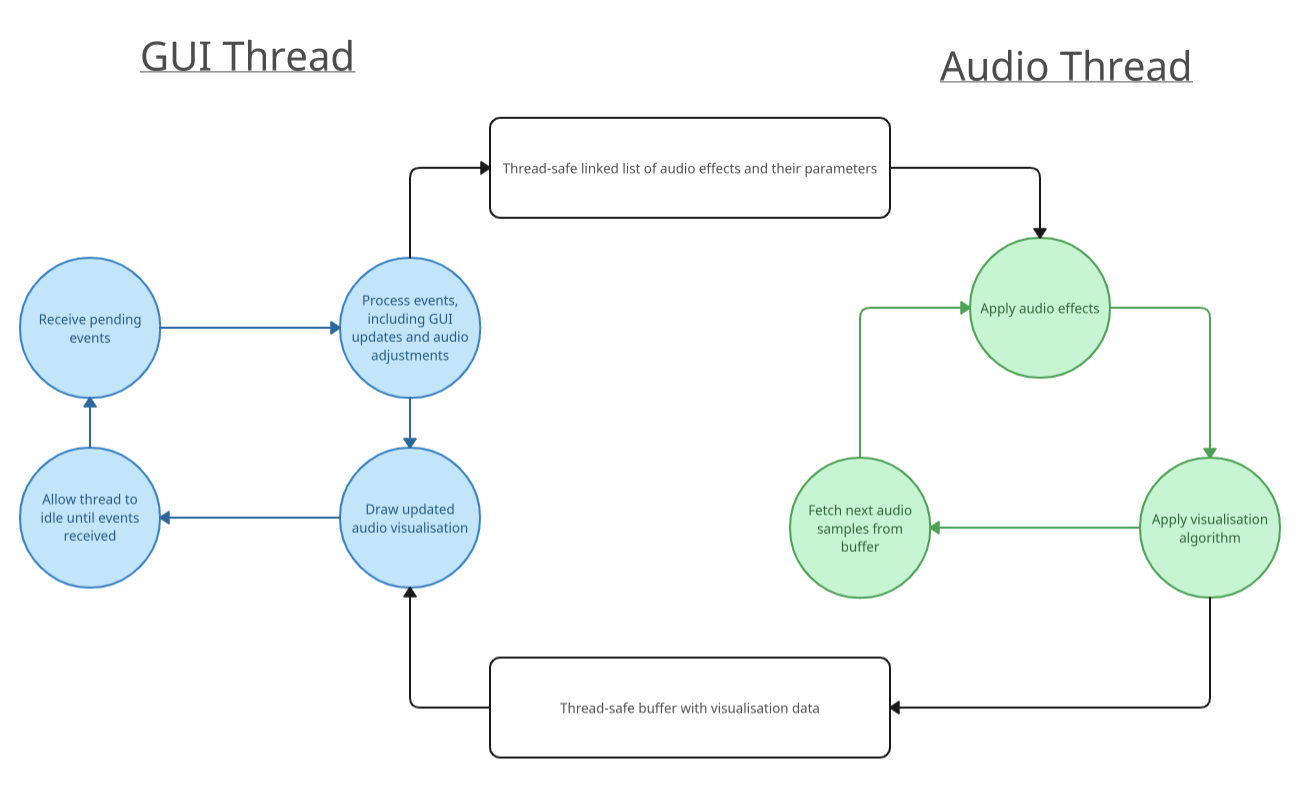
\includegraphics[width=17cm]{threading}
	\caption{Inter-thread diagram - see below for justification for thread-safe data structures}
\end{figure}

\paragraph{}
Typically, GUI programs are written using an event-based paradigm that minimises CPU idle-time. The consequence of this is that, for most of the time, the GUI thread is suspended, awoken only when events from the user (such as mouse clicks or resizing the window) "wake it up". This is desirable in order to minimise system resources used, as more CPU-time will be available for the audio processing requirements, helping to reach the real-time requirements of objective 6. However, this presents a unique challenge. With a single-threaded model:
\begin{itemize}
	\item If the event-based model is followed, the GUI thread is only active when there are pending GUI events to be processed, meaning audio processing can only occur sporadically (resulting in "non-constant" audio)
	\item If instead the GUI thread is constantly active processing audio it will never reach a point where it can process pending events, meaning the program will hang and refuse to process inputs.
\end{itemize}

Hence it is desirable to split the program into two distinct threads. The audio thread can play the audio and perform all necessary processing tasks, whilst the GUI thread can relay input parameters and commands to the audio thread (such as "switch song", "apply effect", etc.).

\paragraph{}
To avoid race conditions\footnote{
	 Race conditions occur when one thread tries to read data whilst the other writes to it. If, for example, the GUI thread removed an audio effect from the audio effect list (see above) and freed it from memory whilst the audio thread was applying that same effect, the audio thread would suddenly be reading from invalid memory, likely resulting in a crash or undefined behaviour.
}, the data that is read by both threads should be thread-safe - only one thread should be able to access the data at a time. This can be achieved by using mutexes\footnote{
	A mutex is an object that prevents multiple threads from accessing data at the same time. It can be thought of as a lock, which can only be unlocked for one thread at a time. They are preferable to spinlocks as they do not require the CPU to waste cycles waiting for the data to be "unlocked", as instead the thread can suspend itself until the mutex becomes available.
}.

\subsubsection{Audio Effects Data Structure}
\paragraph{Picking a data structure} The user will likely want to adjust the order of audio effects at will, and as the same time, it must be very fast to insert and  remove audio effects so as to minimise the time spent not processing audio (even a very short pause may result in "crackles" on weaker hardware). To solve this problem, the audio effects can be stored in a linked list, as unlike std::vectors (dynamic C++ arrays) they prove fast insertion, deletion and swapping irrespective of the number of elements stored.

\paragraph{Making it thread-safe}
To satisfy the requirements of multithreading (see above), I will write my own custom "atomic linked list", backed by a mutex\footnote{
	See above footnote on mutexes
}, which will function just like a normal linked list but maintain thread-safety in all its operations.


\pagebreak

\subsection{Audio Data and Playback}

\subsubsection{Audio Data}
The program will have to load a variety of  user-supplied data in order to operate:
\begin{itemize}
	\item As described in objective 1, the user must be able to load a collection of audio files known as  a "playlist", which will contain the paths of one or more audio files on the system.
	\item Each audio file will consist of a number of audio samples, which will need to be loaded into memory when needed, then freed when not in use.
	\item Audio files also contain other crucial information, such as the audio frequency (e.g. 44,000 Hz), the number of channels (usually mono (1) or stereo (2)), and the number of samples (the "length").
	\item Thus to keep track of the audio files loaded into memory, each audio file will need to store its raw audio samples, its frequency, the number of channels, and the number of samples.
\end{itemize}

\subsubsection{ Audio Data UML }
\begin{figure}[H]
	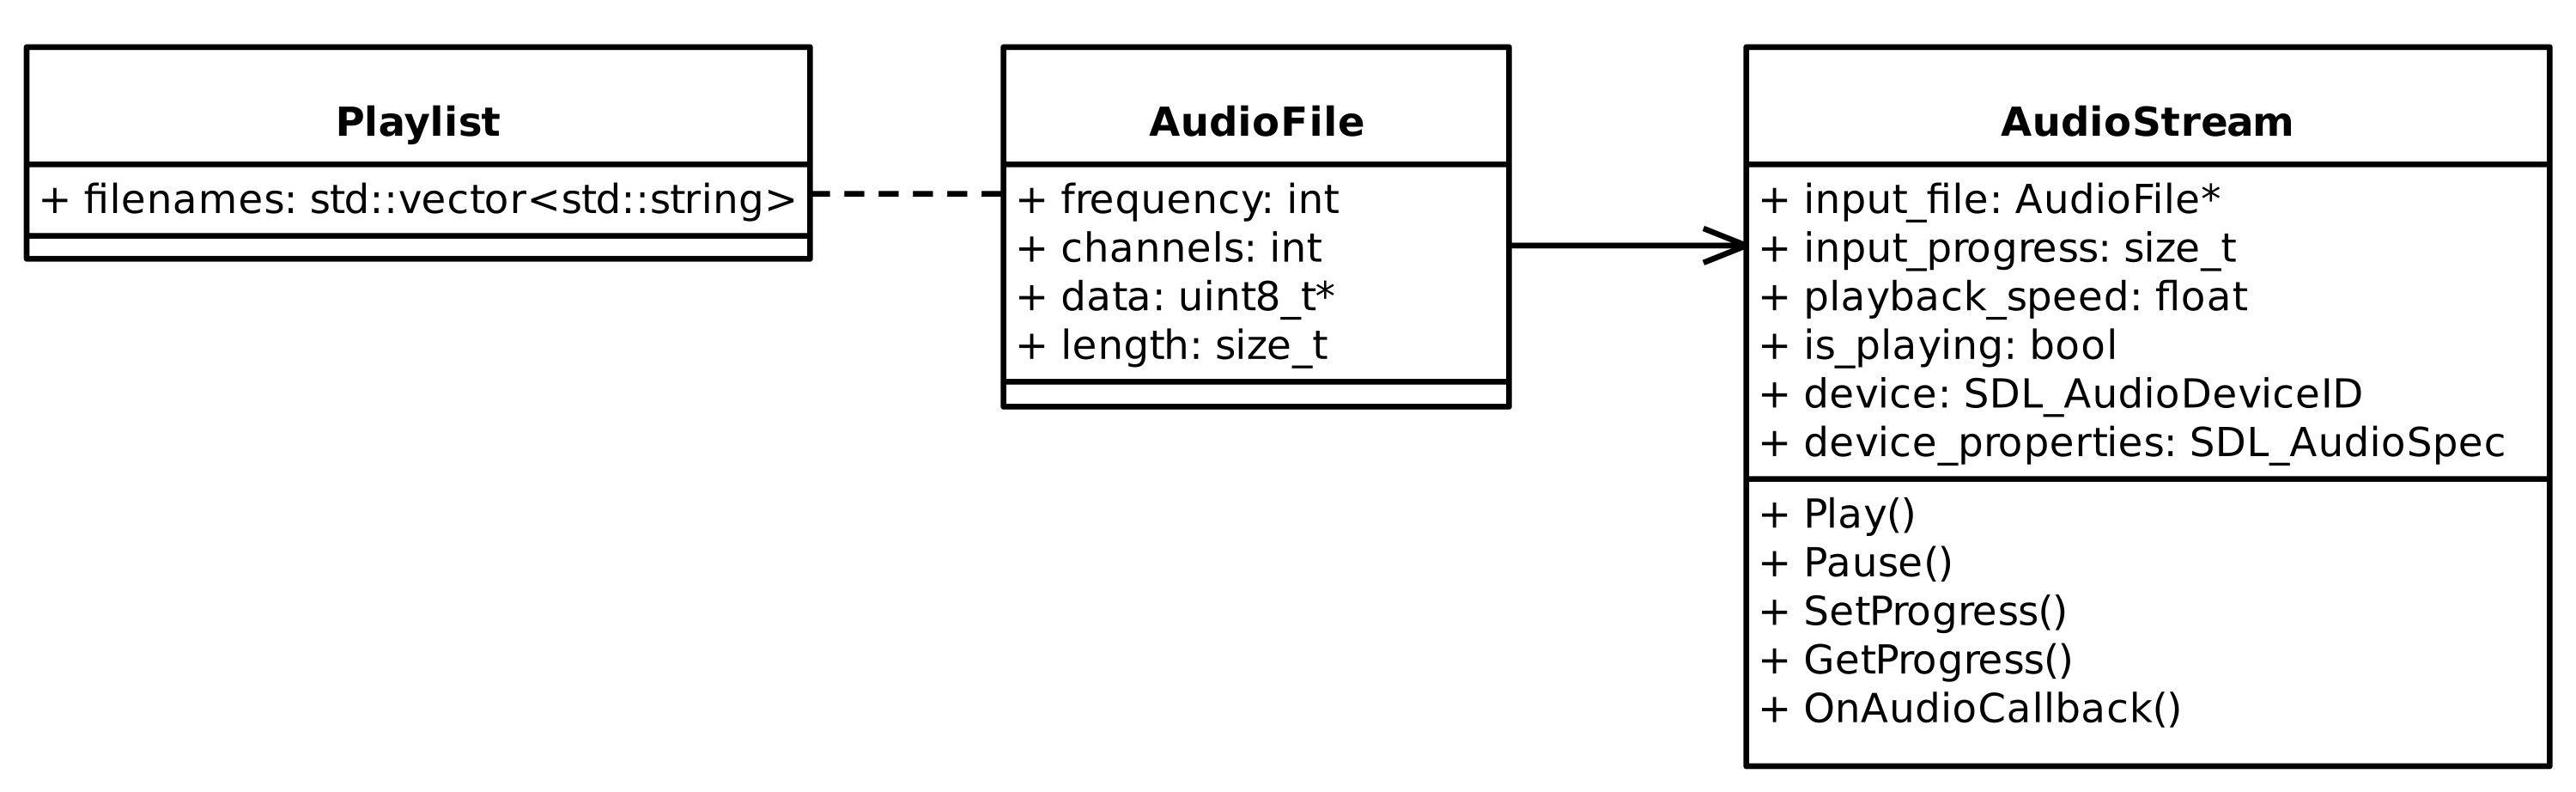
\includegraphics[width=14cm]{audio io uml}
	\caption{UML for Audio Data and IO - separate getter and setter exists for AudioStream progress as the caller will express progress as percentage (e.g. 50\% played) so that it is independent of file size. The playlist contains the filenames of all audio files on disk, and an AudioFile instance is created, when needed, by loading the audio file from disk using this filename. }
\end{figure}

\subsubsection{The Need for Streaming}
It may be tempting to load and unload all audio data in a hierarchal  fashion as such:
\begin{enumerate}
	\item An attempt is made in the code to load a playlist.
	\item To do this, the playlist will be read from disk and all the audio file paths contained within will be loaded into memory.
	\item Each audio file path will be verified to check it is valid exists on the system.
	\item If the playlist is valid, each audio file will then be loaded using the paths provided.
	\item Thus the loading of a playlist will involve loading all audio files referenced within.
	\item At the end of the program, when the playlist is no longer needed, all the playlist's audio files will be freed from memory, followed by the playlist itself.
\end{enumerate}

However, this is not a practical approach due to memory usage constraints. If a user attempted to load a playlist consisting of 200 songs, each 5 MB each, this would consume roughly 1000 MB of memory for the entire duration of the program, even though only 1 audio file can be played at once (and hence only one needs to be in memory at any one time). This conflicts with objective 6 ("the system must run in real-time on an average school computer") as many computers may not have large amounts of free memory, particularly if other programs are running, which may lead to an out-of-memory crash. 

\paragraph{}
Instead, I have decided to "stream" audio files as they are played, so that only the audio file currently needed is resident in memory. This can be modelled as followed:
\begin{enumerate}
	\item An attempt is made in the code to load a playlist.
	\item To do this, the playlist will be read from disk and all the audio file paths contained within will be loaded into memory.
	\item Each audio file path will be verified to check it is valid exists on the system. If the playlist is valid, the execution of the program will continue.
	\item Each time the next audio file is to be played from the playlist, the program will dynamically load it from disk (using the path from the playlist) and store it in memory.
	\item When the next audio file is chosen, it is loaded as described above. Crucially however, the previous audio file is first unloaded from memory, as it is no longer needed.
	\item At the end of the program, the currently playing audio file and playlist are both freed.
\end{enumerate}

\paragraph{}
In this way, the issue of large playlists resulting in extremely large memory consumption will be avoided, as only one audio file will be loaded at once. 

\subsubsection{Audio Playback}
The playback of audio itself presents many challenges. In order to make the code as modular and decoupled as possible, I will abstract away the low-level creation of audio devices, pausing, un-pausing, etc. into an "AudioStream" class. One will simply create an "AudioStream", supply it with data, and the class will manage the various complexities of multithreading and feed the audio buffer with data at the appropriate times.

\paragraph{}
In order to maximise portability of the code,  and hence make it as cross-platform as possible in order to maximise the program's audience, I have decided to use a library called "SDL2" to handle audio playback, as it abstracts away the native APIs one would have to otherwise use. In this way, separate audio code does not have to be written for Windows, Linux, etc.

\paragraph{}
The code that plays audio on the system will run on a separate thread (see multithreading section). This audio thread is invoked at regular intervals by the operating system by way of a "callback" function. When this happens, it is the program's responsibility to supply the operating system with the next buffer of audio. This is summarised below:

\begin{enumerate}
	\item An "AudioStream" is created and supplied with the raw audio samples from the audio file, as well as pointers to the atomic linked list of audio effects and to the visualisation data buffer.
	\item The AudioStream uses SDL2 to invoke audio playback at regular intervals on a separate thread (the "audio thread") using a callback
	\item Every time the callback is called, the AudioStream will fetch the next section of upcoming audio that it has been supplied with.
	\item Each audio effect will then be applied (using the audio effects atomic linked list).
	\item The audio visualisation module will then be invoked on the audio just processed, and its output written to the visualisation data buffer.
	\item Now that all work is done for the current section of audio, the processed audio will be copied to the callback's audio buffer and the audio thread will suspend itself.
	\item When the next section of audio is due, the callback will be re-invoked.
\end{enumerate}

\subsubsection { Audio Playback Flowchart }
\begin{figure}[H]
	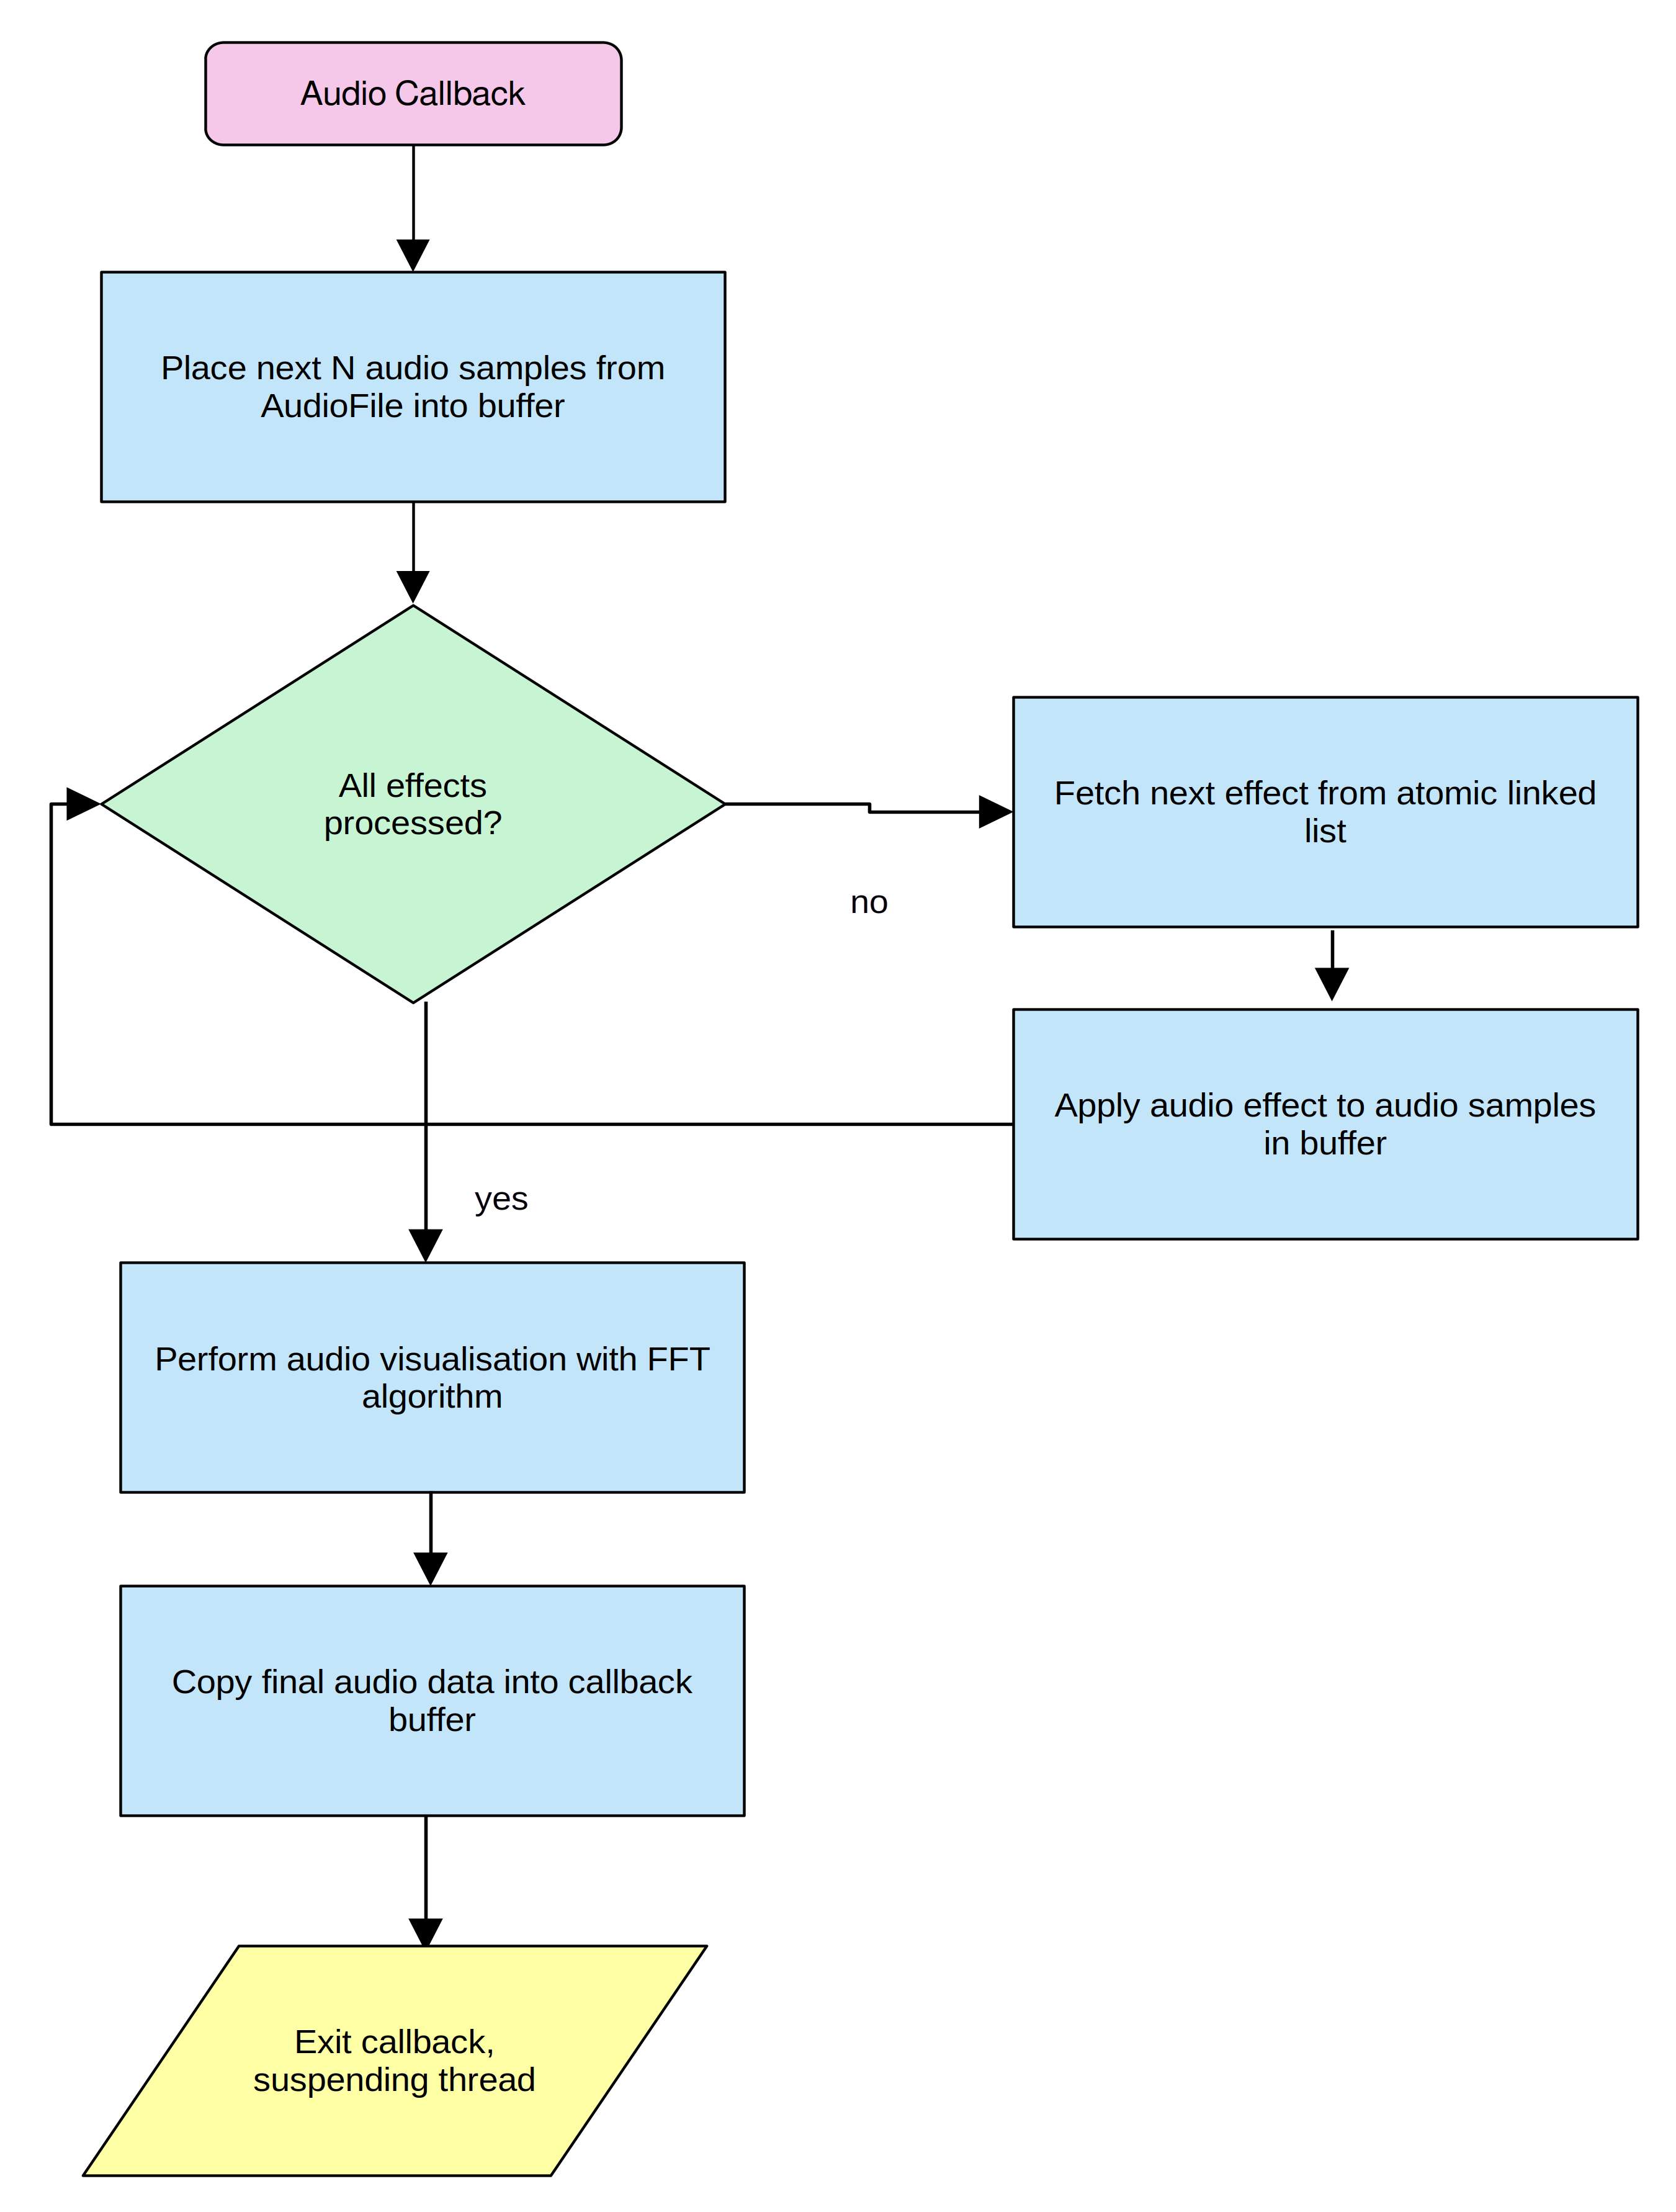
\includegraphics[width=14cm]{audio io flowchart}
	\caption{Flowchart for AudioStream's SDL audio device callback}
\end{figure}

\pagebreak

\subsection{Audio Effects Architecture}
The full list of audio effects detailed in the analysis section is as follows:
\begin{itemize}
	\item Equaliser (frequency modification) - selectively modifying frequencies such as by performing a bass boost
	\item Echo - making audio sound like it's recorded in a large room
	\item Volume adjustment - modifying the amplitude of the audio
	\item Noise - adding subtle imperfections to the audio
\end{itemize}

\subsubsection{Unique Audio Effect Traits}
Each audio effect will need its own properties, and potentially its own mutable state (for example, the echo effect needs to "remember" the previous audio samples so it can repeat them later). Below is a summary of the requirements, properties and state of each audio effect.

{
\renewcommand{\arraystretch}{1.5}
\begin{table}[h!]
	\begin{center}
		\begin{tabularx}{1.0 \textwidth} {
				| >{\raggedright\arraybackslash}X 
				| >{\raggedright\arraybackslash}X
				| >{\raggedright\arraybackslash}X 
				| >{\raggedright\arraybackslash}X  |
			}
			\hline
			Effects & Requirements & Properties & State \\
			
			\hline
			Equaliser & Allow the user to alter the volume of a selected frequency range. Multiple equaliser effects can be applied successively to cover multiple ranges.  & Lower frequency \newline  Upper frequency \newline Multiplier  & None \\
			
			\hline
			Echo & Produce an echo effect where audio sounds like it's getting reflected in a large room & Fall-off (how quickly echoes fade) \newline Delay samples (how many samples must pass before a sample is echoed) & Previous audio samples buffer \\
			
			\hline
			Volume & Adjust the volume / amplitude of incoming audio & Volume multiplier & None \\
			
			\hline
			Noise & Add subtle imperfections to the audio & Intensity (the volume of the noise) & None\\
			
			\hline
		\end{tabularx}
	\end{center}
\end{table}
}

\subsubsection{Common Audio Effect Traits}
Immediately it is obvious that all audio effects will share many common features. Each effect shall:
\begin{itemize}
	\item Take a number of audio samples as input
	\item Have a number of configurable options which need to be exposed to the GUI front-end
	\item Perform processing on all audio samples at once
	\item Output its final processed audio
\end{itemize}

\paragraph{}
Given these requirements it is wise to use an object-orientated inheritance approach where effect subclass inherits from a common parent, which provides common functionality (such as the storage and exposing of configuration options), as well as providing a common interface that other parts of the code can use. In order to abstract away the details of interacting with an audio effect, two new classes will also be needed.

\subparagraph{Packet} A packet represents a chunk of audio awaiting processing by the effect. However, some effects require knowledge of both the previous audio samples and future audio samples (like echo). Thus, each packet will consist of 3 audio buffers - one for the previous, current and next buffer of audio samples. A packet will also contain the frequency of the incoming audio as this is required for the FFT maths.

\subparagraph{Property} Each audio effect has a number of configurable properties. To aid in validation, each property will have a current,  minimum and maximum value, as well as a flag to differentiate between integer values and decimal values.

\paragraph{}
Both these classes will be independent of the main audio effect parent class. The audio effect parent class will merely use these classes to represent the data provided and stored by it. This is an example of {\it composition}.

\subsubsection{Properties Data Structure}
Each audio effect will have a list of properties. When drawing a properties GUI, the front-end code will want an easy and convenient way of both getting a list of all available properties, along with their respective names. In a similar fashion, when setting the values of certain properties, it will be most convenient if properties can be accessed using their names.

\paragraph{}
I will use a hash-map as my data structure for this purpose. Hash-maps can be indexed by using the name of the property (e.g. "minimum frequency" as the key), simplifying the front-end code and avoiding the need for a separate "property name" variable. In addition, they provide very fast look-up with an O(1) time. Whilst hash-maps are expensive when it comes to adding and removing elements, each audio effect will only have a fixed number of properties so this will not be an issue.

\subsubsection{UML Class Diagram}
After considering all the requirements of the multiple classes required, I have constructed a class diagram. However, a slight modification has been made to the typical UML structure: properties of audio effects are prefixed with an * (asterisk) in order to indicate that their are not attributes {\it per se}, but rather are elements in their parent's properties hashmap.

\begin{figure}[h]
	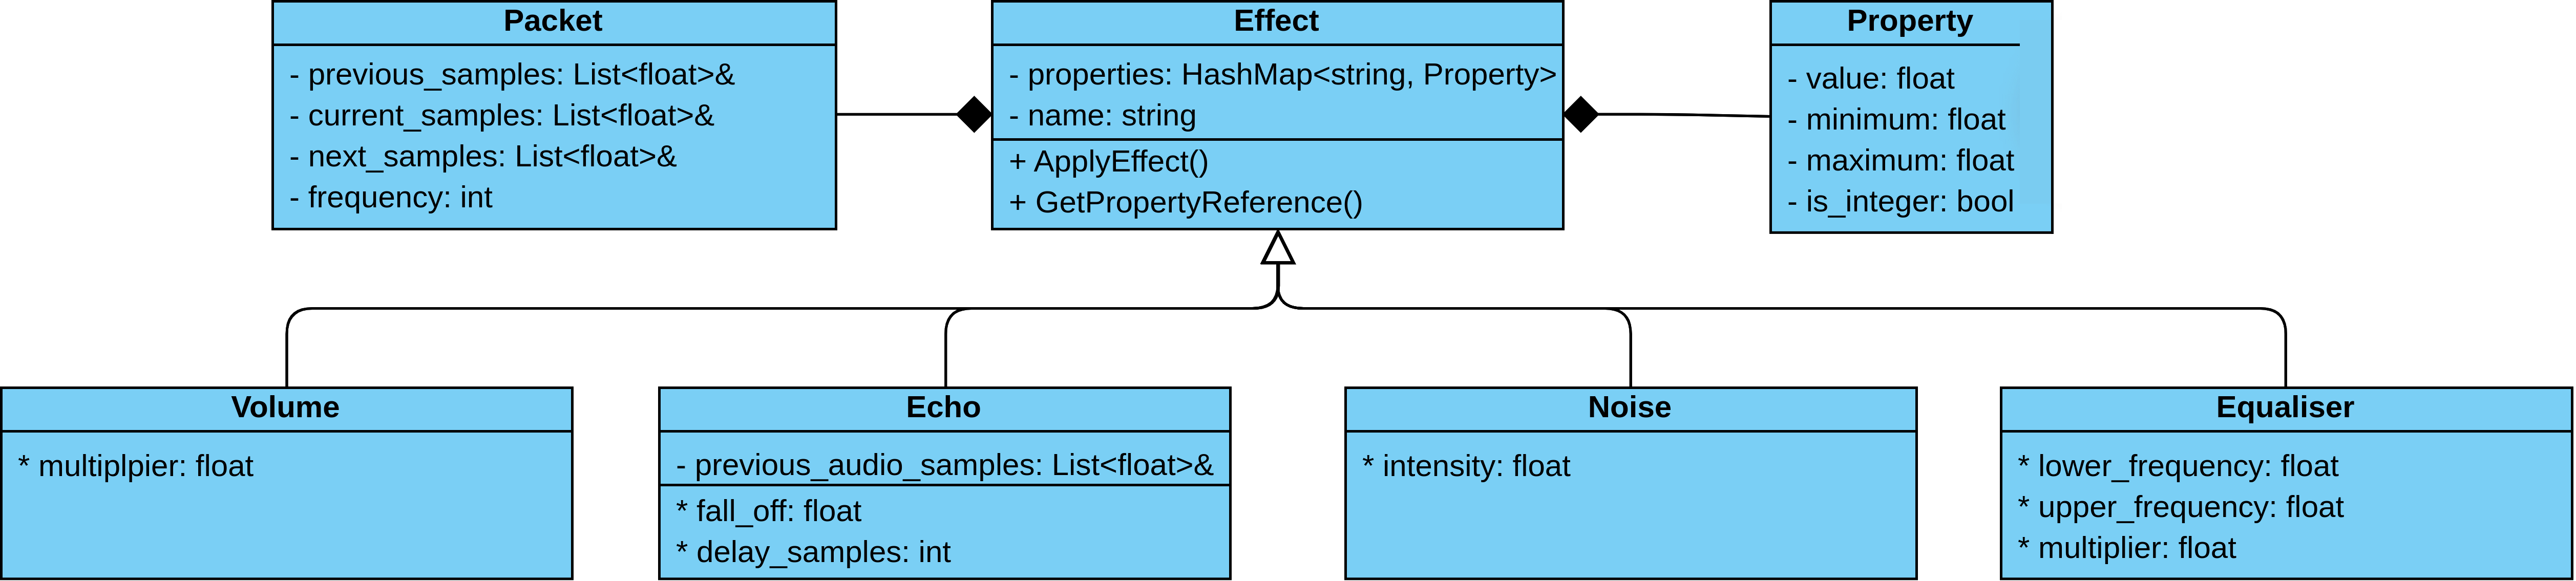
\includegraphics[width=\textwidth]{effects class diagram}
	\caption{UML class diagram containing attributes, operations and custom "properties"}
\end{figure}

\pagebreak

\subsection{High-Level Audio Effects Flowcharts}
\begin{figure}[H]
	\subsubsection{Equaliser}
	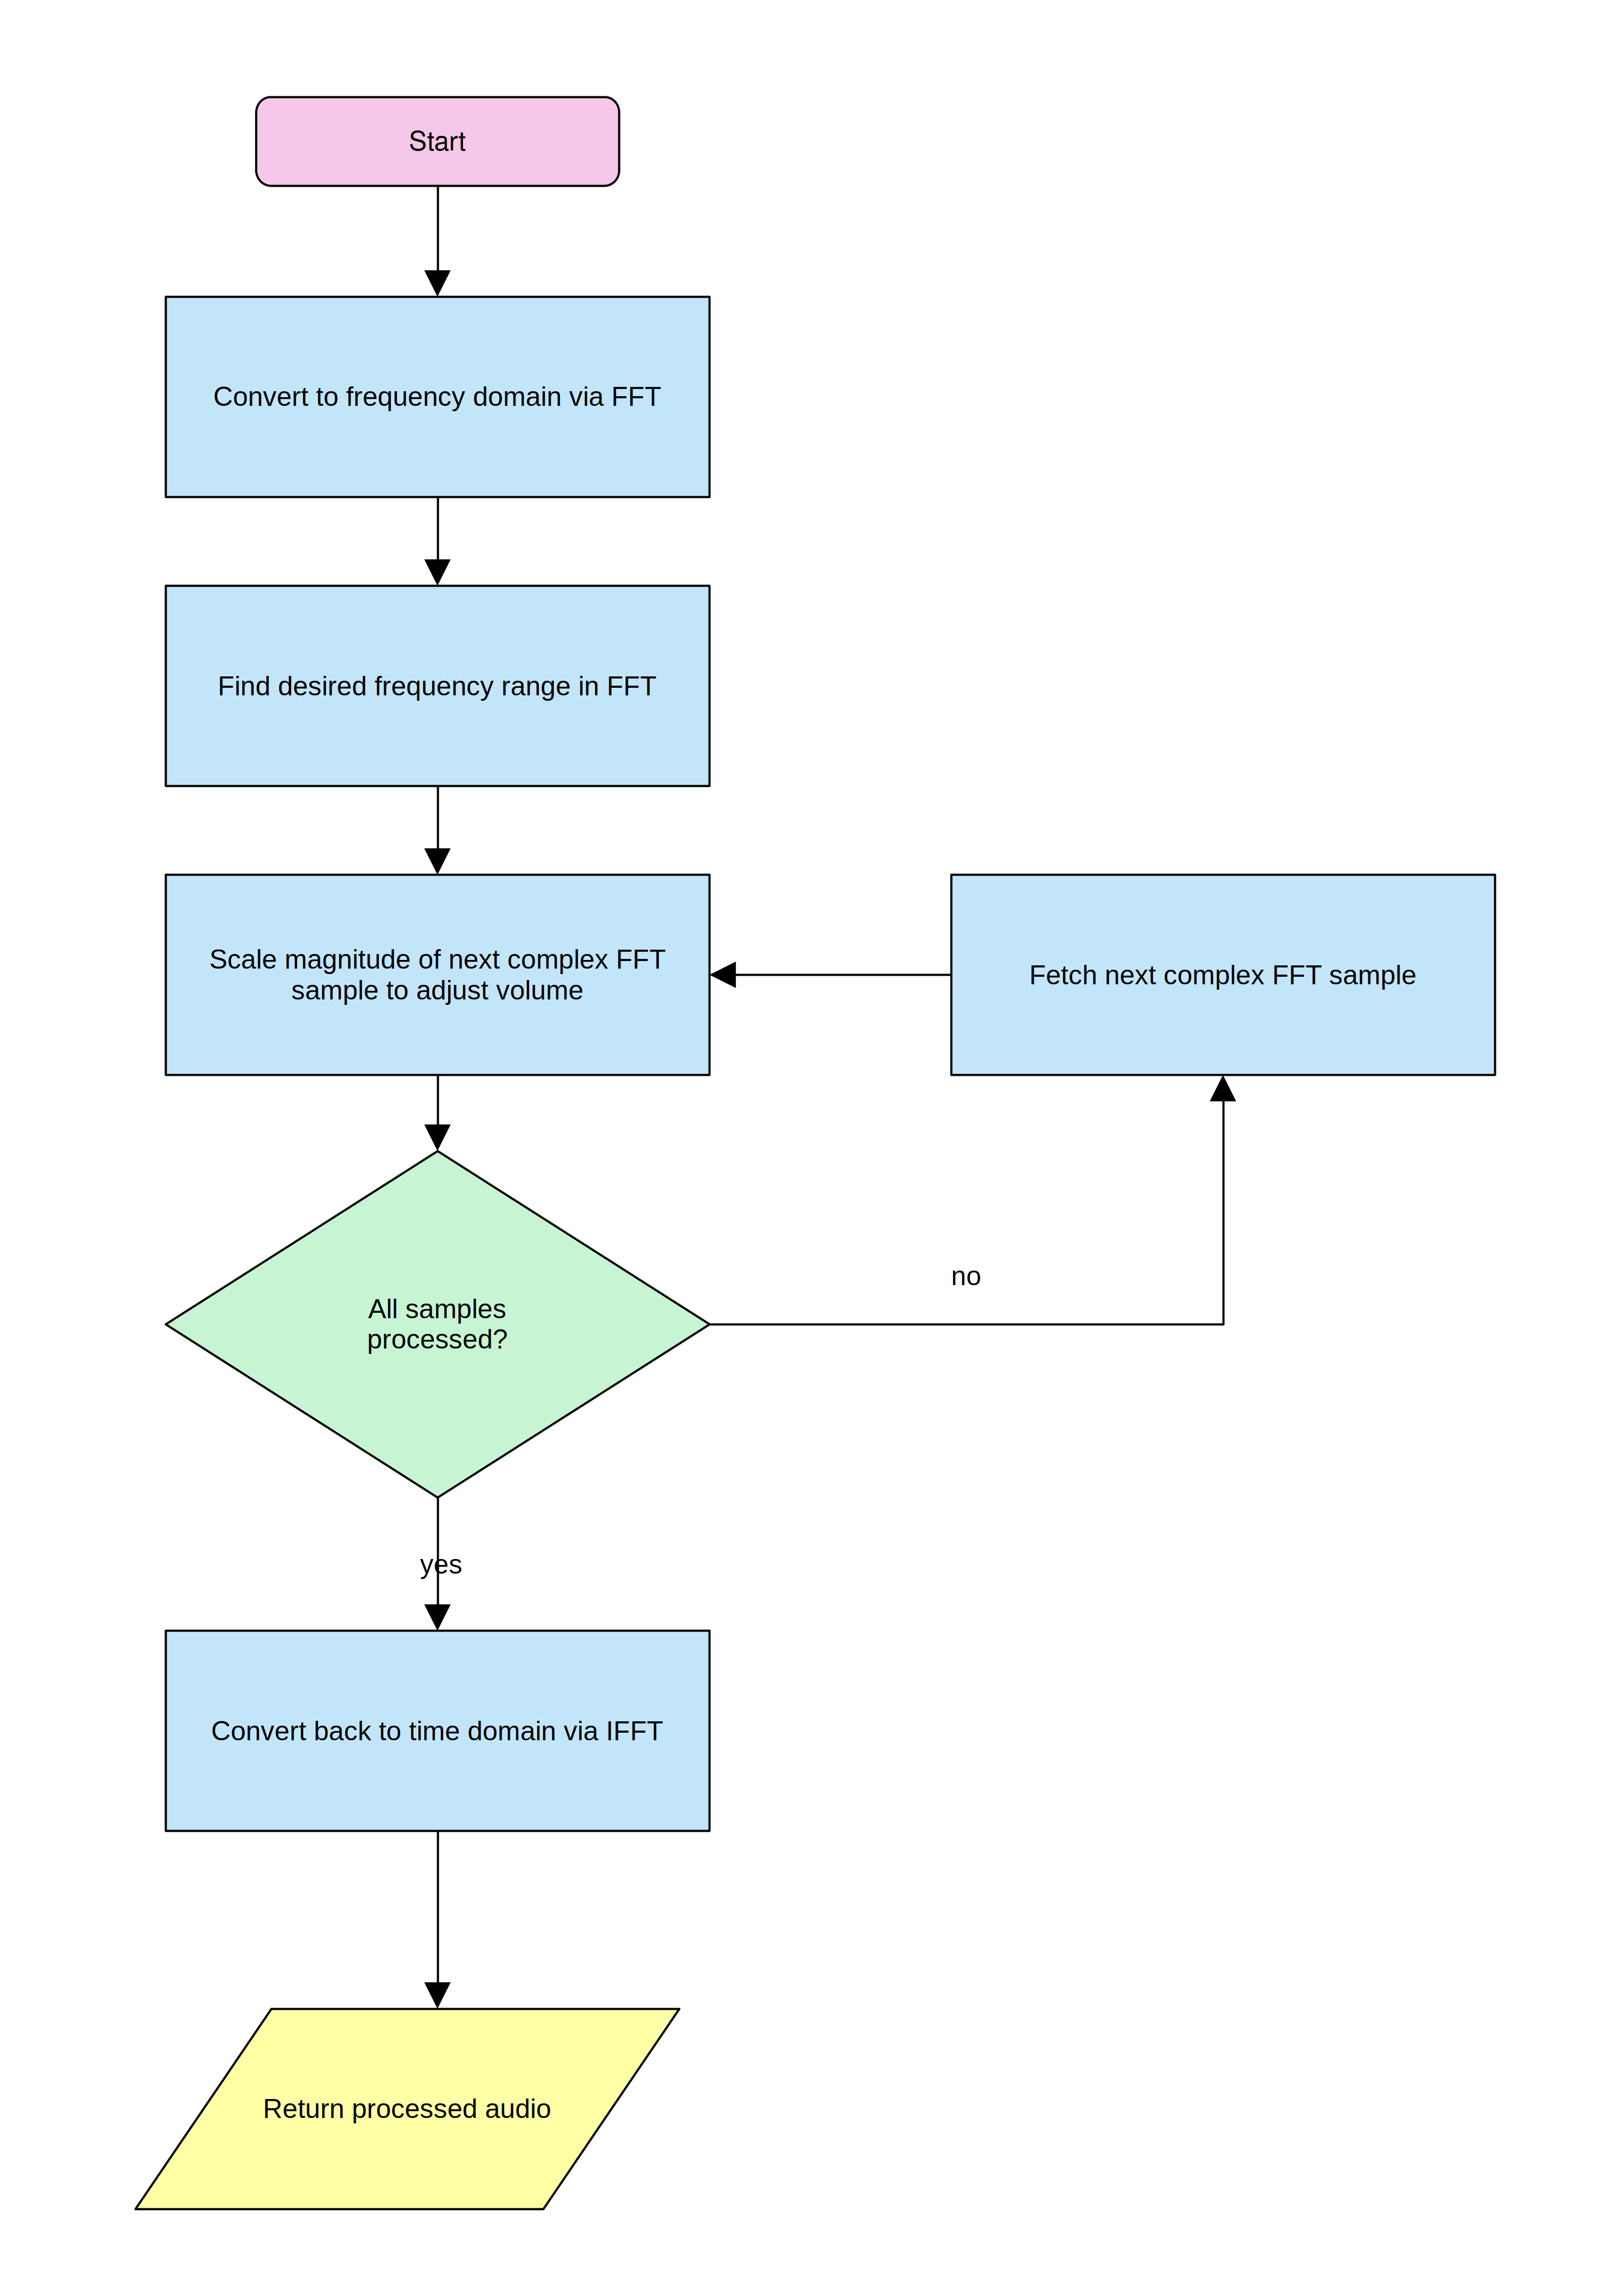
\includegraphics[width=14cm]{equaliser flowchart}
	\caption{Flowchart for equaliser (frequency modification) audio effect}
\end{figure}

\begin{figure}[H]
	\subsubsection{Echo}
	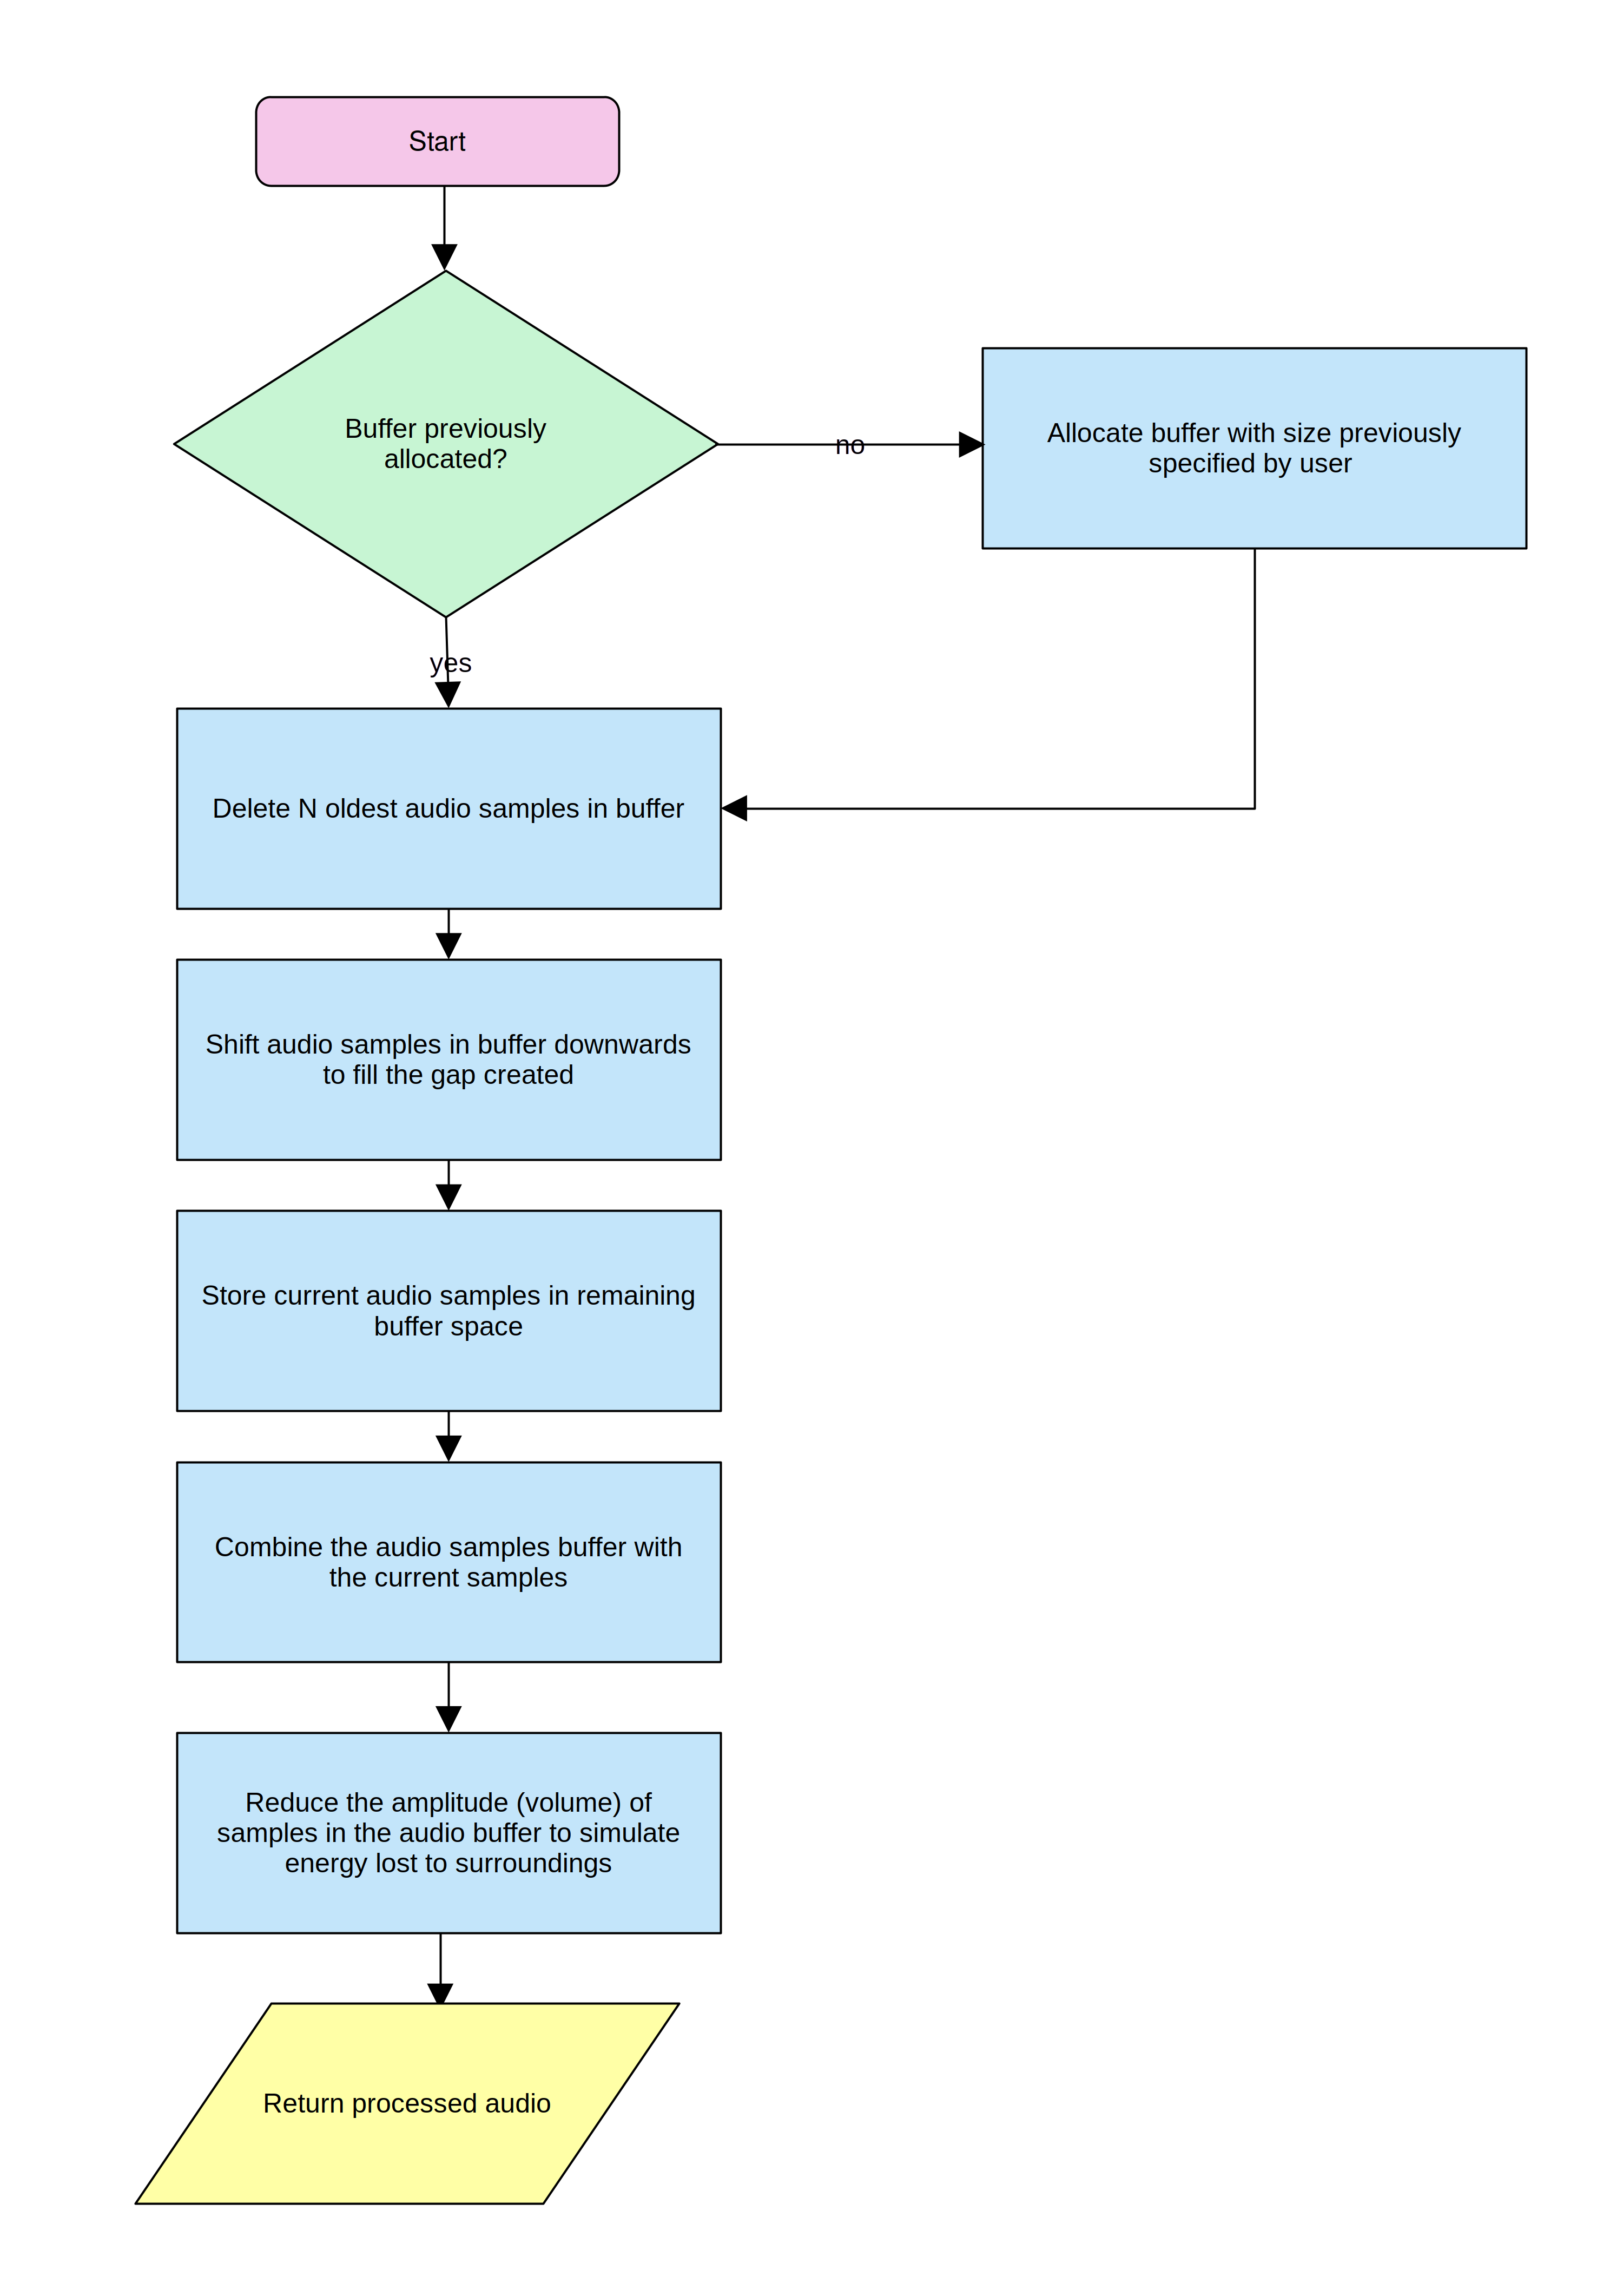
\includegraphics[width=14cm]{echo flowchart}
	\caption{Flowchart for echo audio effect}
\end{figure}

\begin{figure}[H]
	\subsubsection{Volume}
	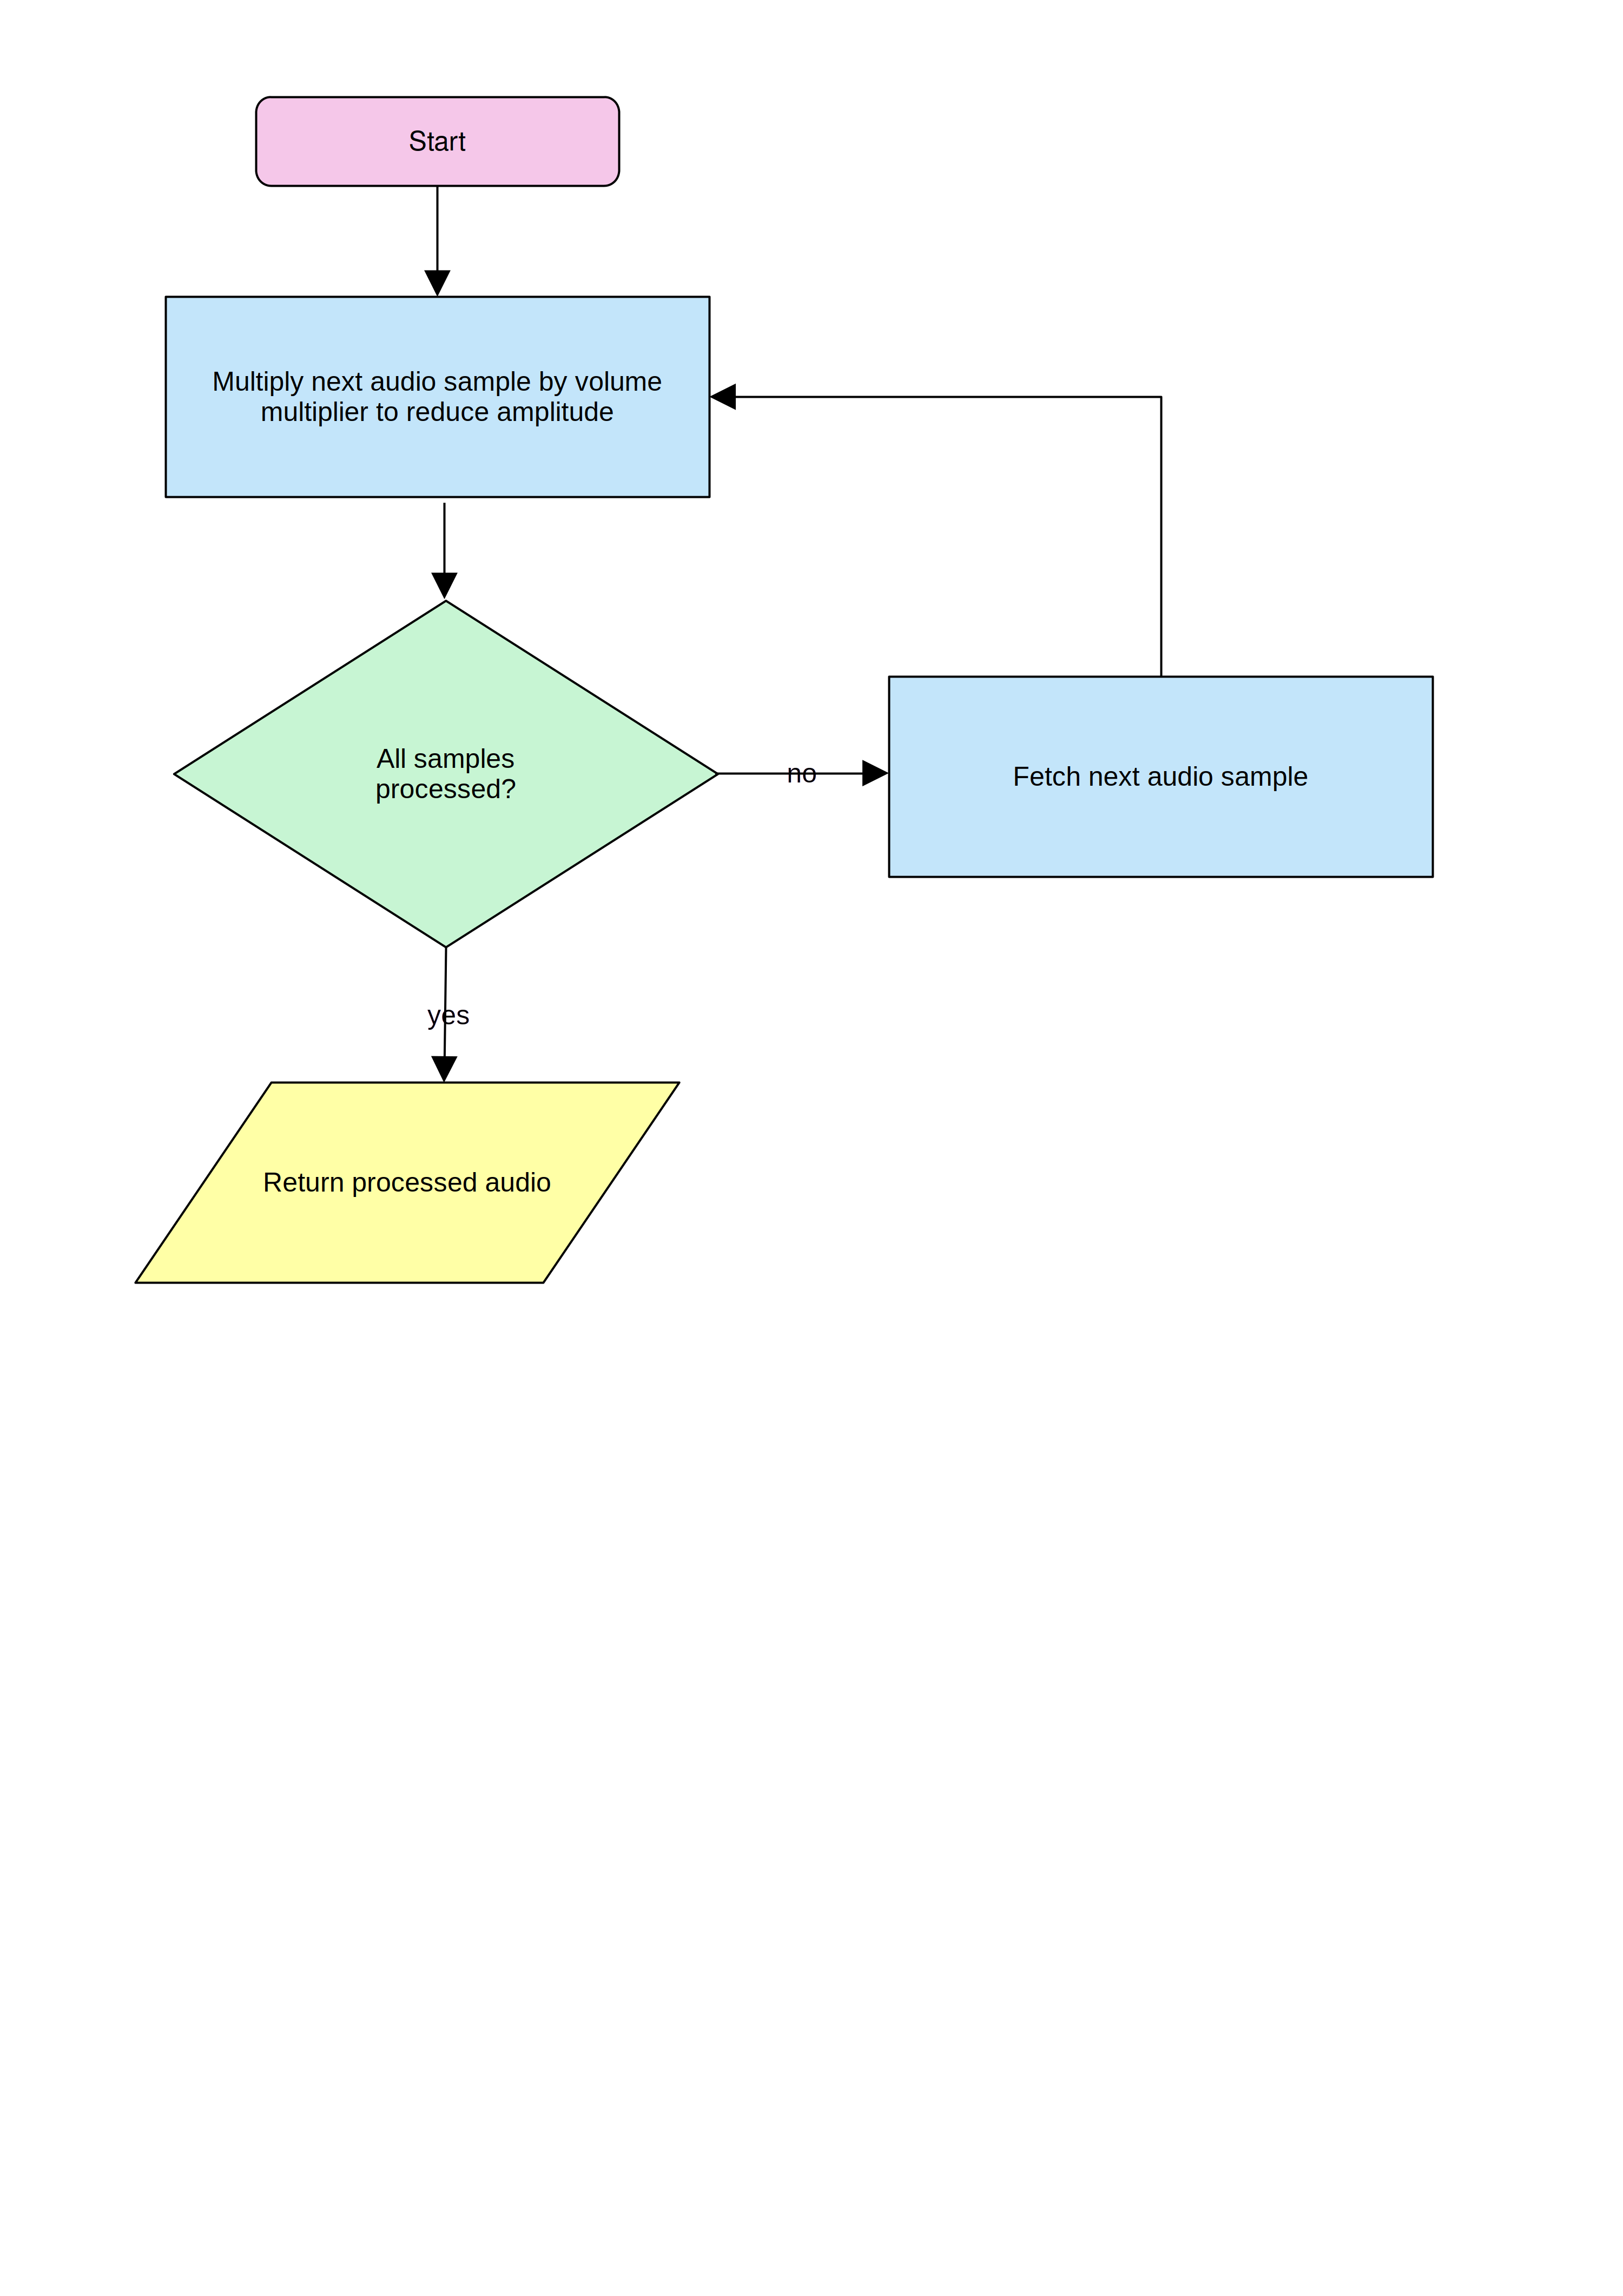
\includegraphics[width=14cm]{volume flowchart}
	\caption{Flowchart for volume audio effect}
\end{figure}

\begin{figure}[H]
	\subsubsection{Noise}
	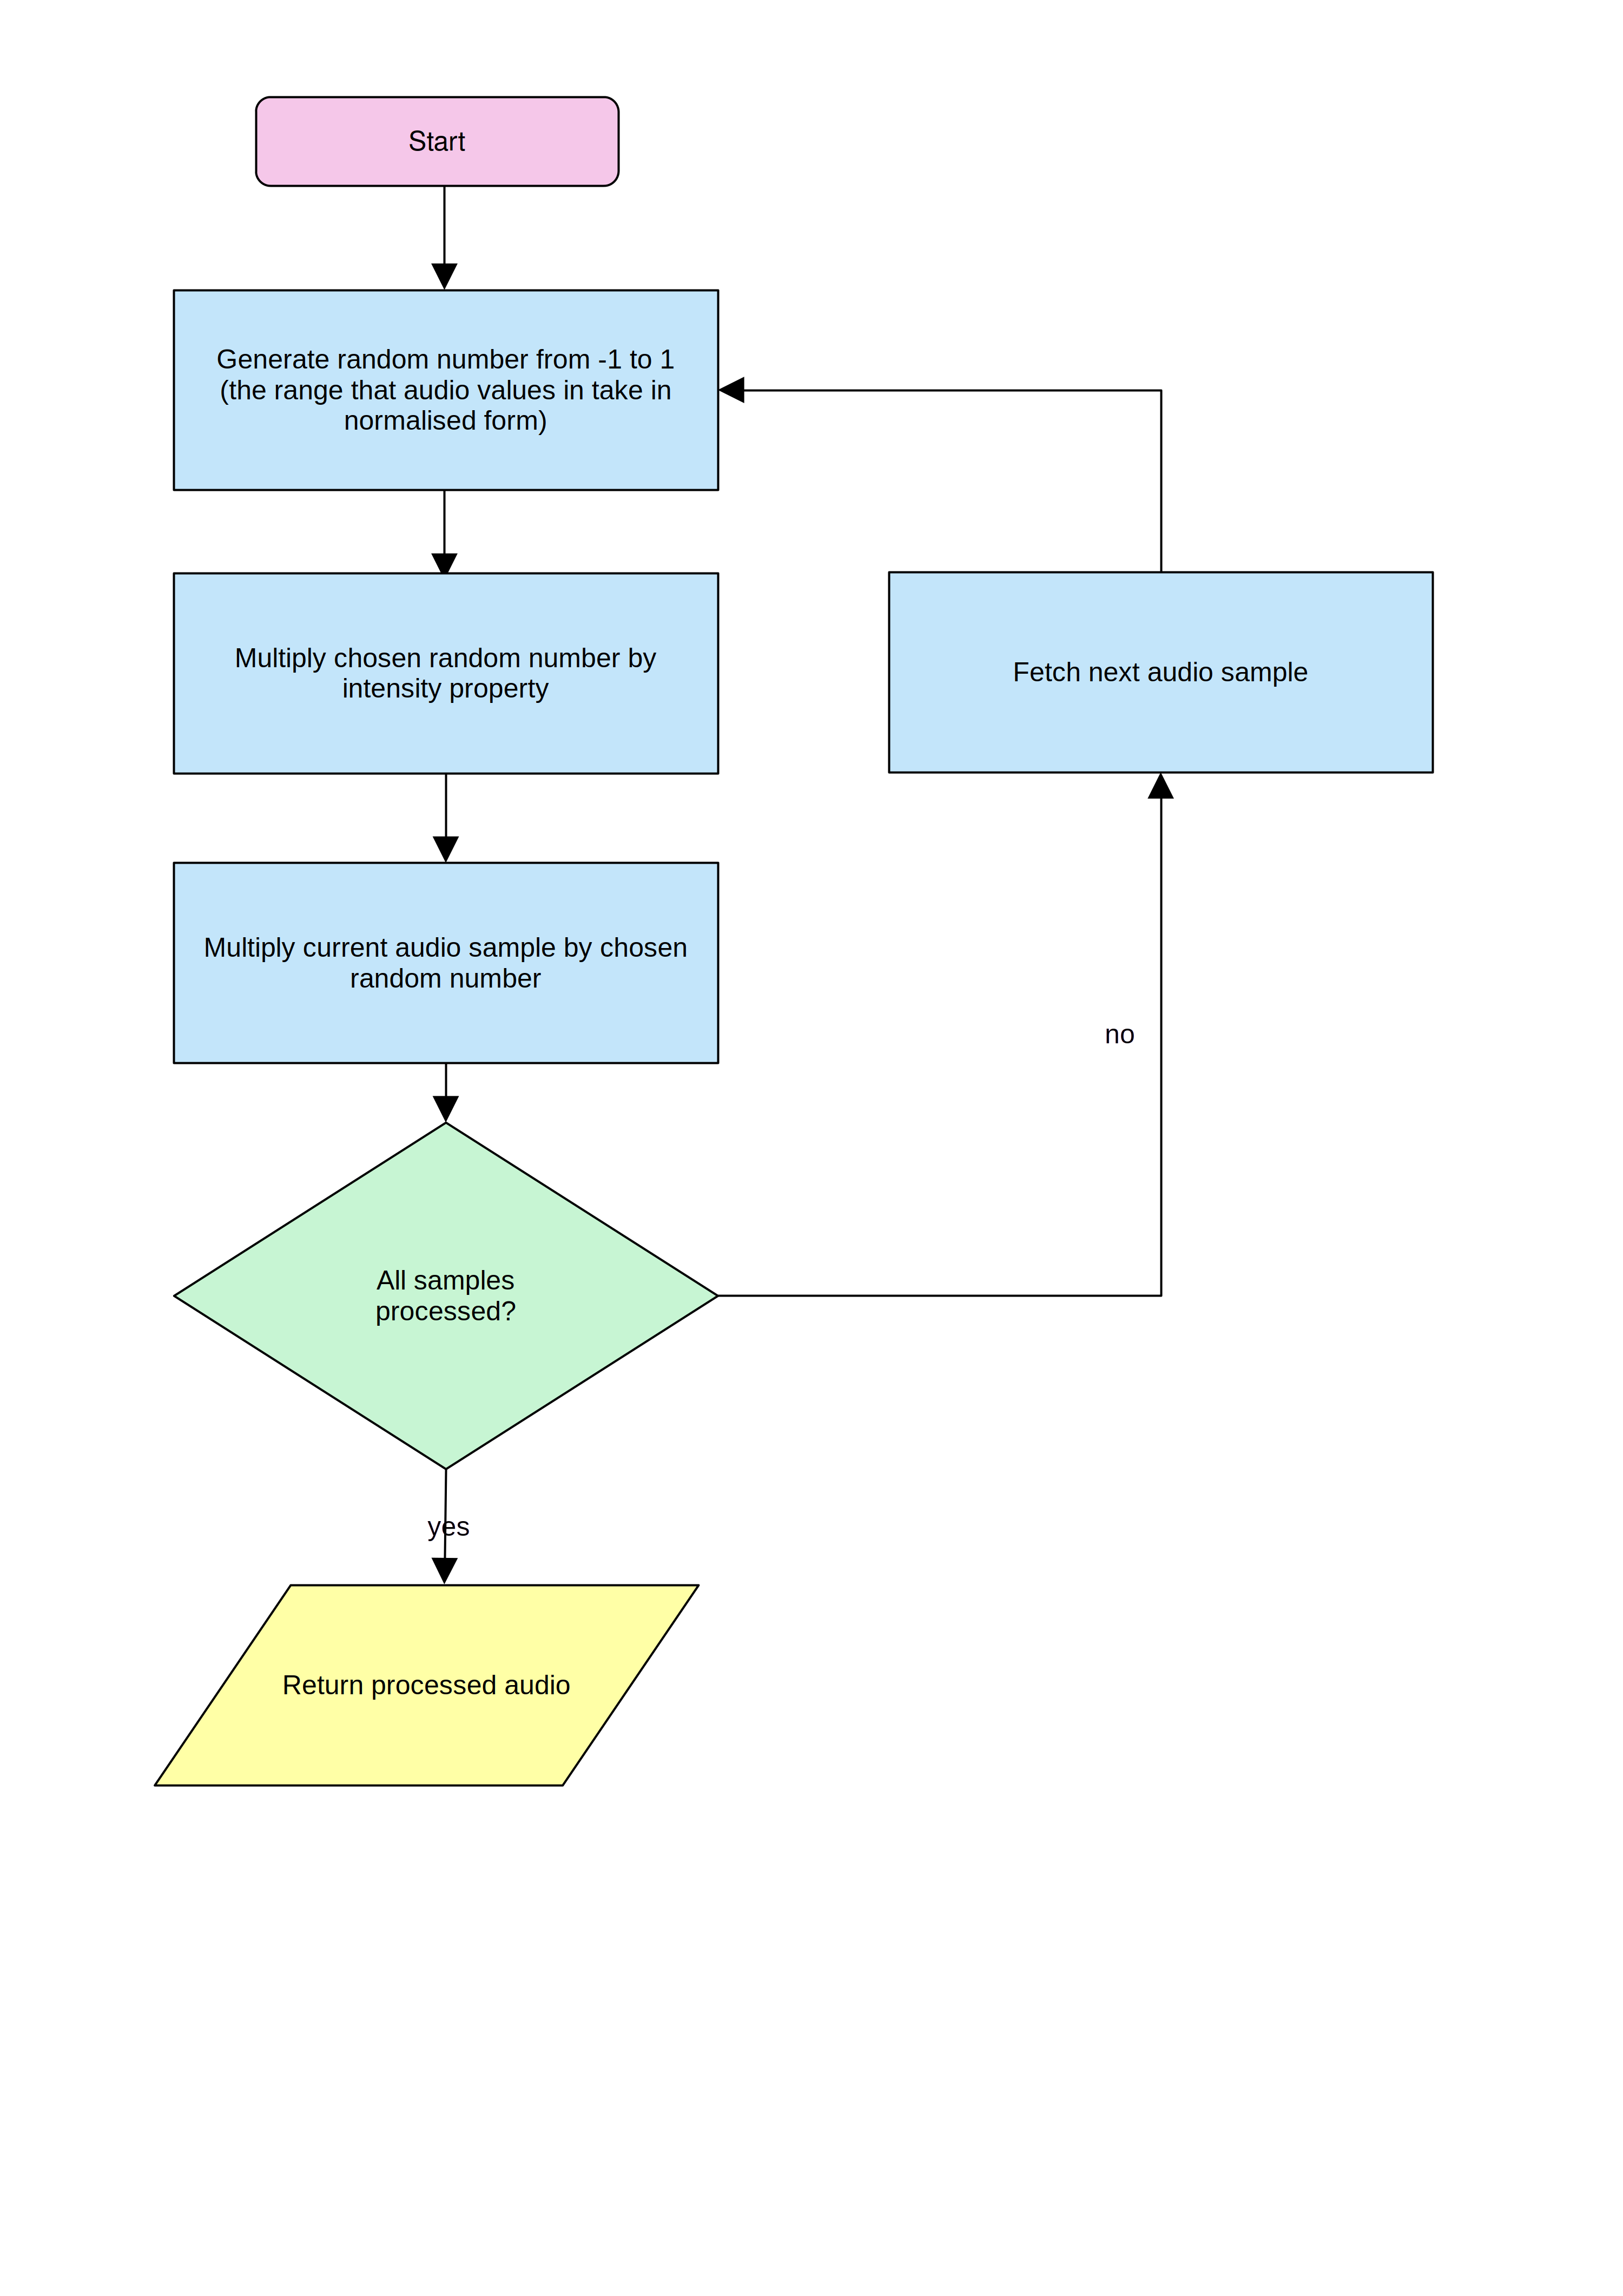
\includegraphics[width=14cm]{noise flowchart}
	\caption{Flowchart for noise audio effect}
\end{figure}

\pagebreak
\subsection{Program GUI}

\paragraph{}
The user will interact with the program using a GUI. In order to maximise the potential user-base, I have decided to use a popular C++ GUI library called "wxWidgets", which allows for the creation of GUIs using a singular code-base for Windows, Linux and MacOS, amongst others.

\subsubsection{GUI "screens"}
The user will navigate through a variety of "screens" in order to use the program. The GUI flow can be modelled as followed:
\begin{itemize}
	\item When the program starts, the user must chose to either load an existing playlist (see "Audio Data and Playback"), or create a new one - this is the "choice screen".
	\item Should the user chose to create a playlist, a new "screen" will be displayed where they can append audio files on the system to a playlist, before saving it.
	\item Returning back to the initial "choice screen", the user will then chose to load their existing playlist, or optionally create another one for later use.
	\item After a playlist has been selected, the main "playback screen" will be displayed. Audio playback will begin.
	\item The user can view the current audio visualisation, as well as audio playback progress.
	\item A menu will allow the user to configure the current playback and visualisation, such as by adding new audio effects or changing the visualisation settings.
	\item A separate "screen" can be displayed allowing the user to view current audio effects.
	\item In this screen, if a user chooses to edit a current audio effect, a new screen will be displayed, showing the various options one can adjust.
\end{itemize}

\paragraph{Summary of "screens"}
\begin{itemize}
	\item "Choice" screen (create new playlist or load existing one)
	\item "Create playlist" screen
	\item "Playback" screen
	\item "Effects list" screen
	\item "Edit effect" screen
\end{itemize}

\paragraph{Popups}
Minor tasks such as  selecting a new song from a playlist or modifying visualisation settings will be handled with popup dialogue menus.

\begin{figure}[H]
	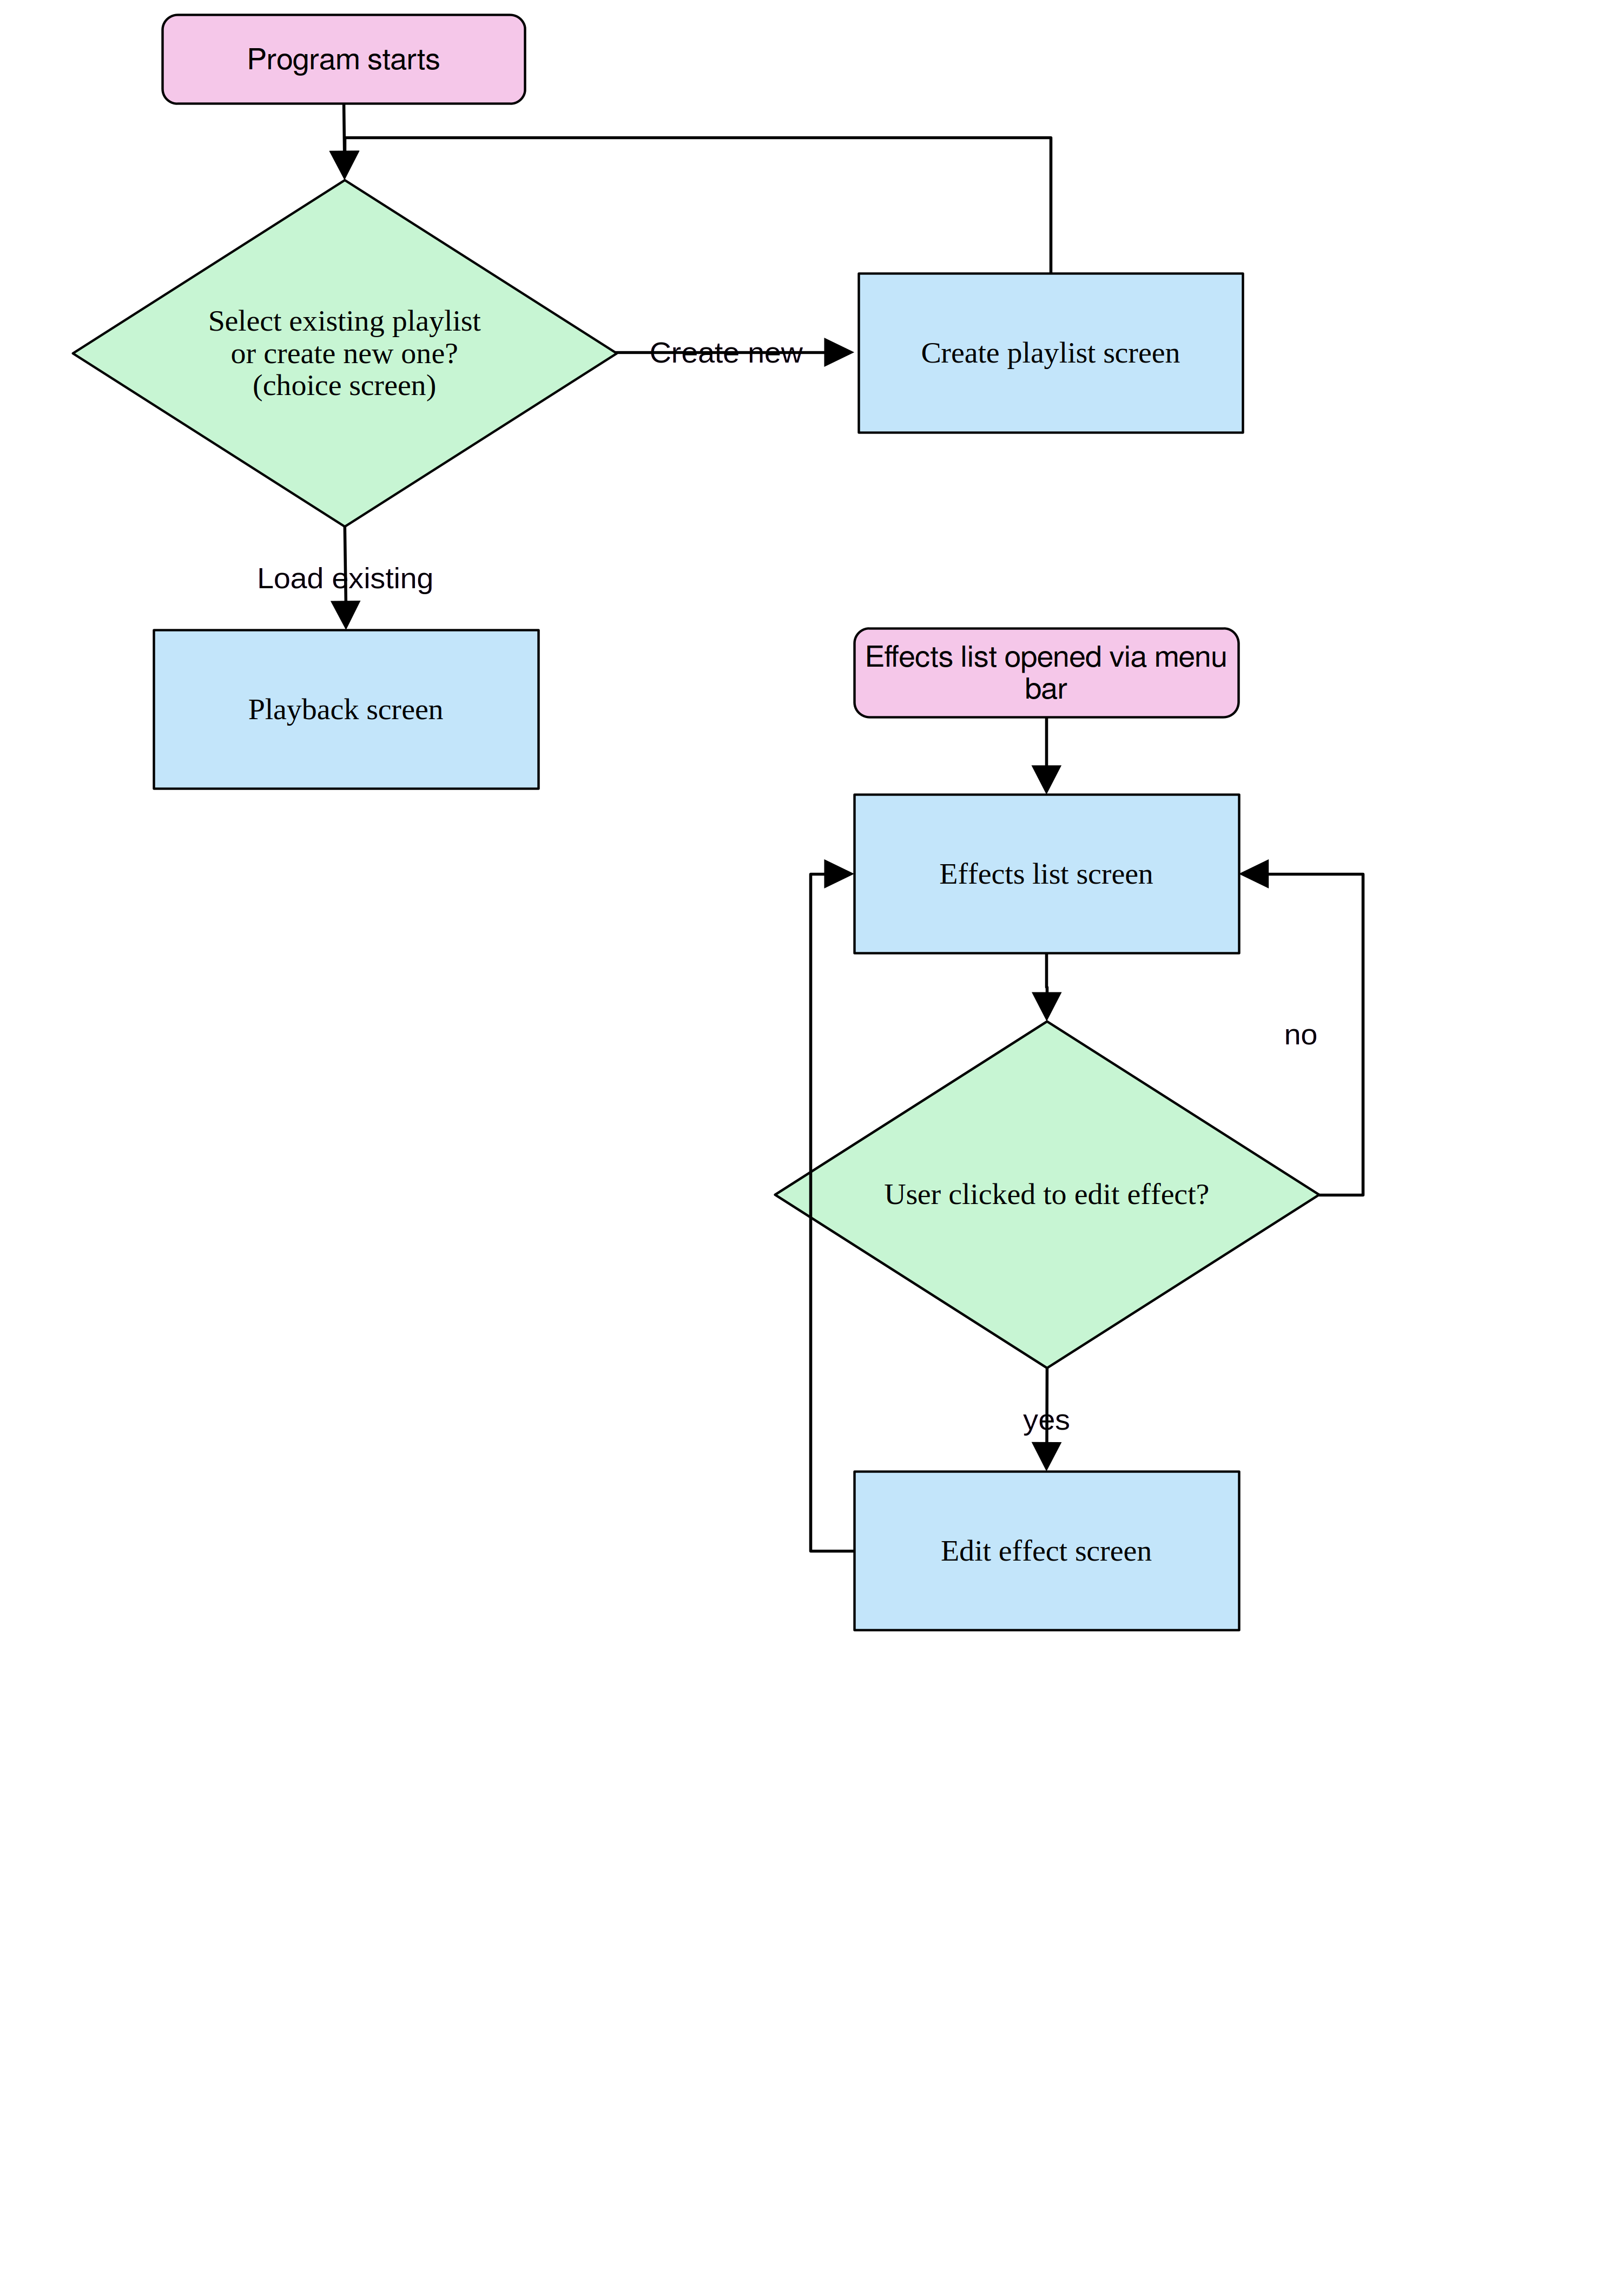
\includegraphics[width=14cm]{gui flow}
	\caption{GUI flow for program }
\end{figure}

\subsubsection{GUI Wireframes}

\begin{figure}[H]
	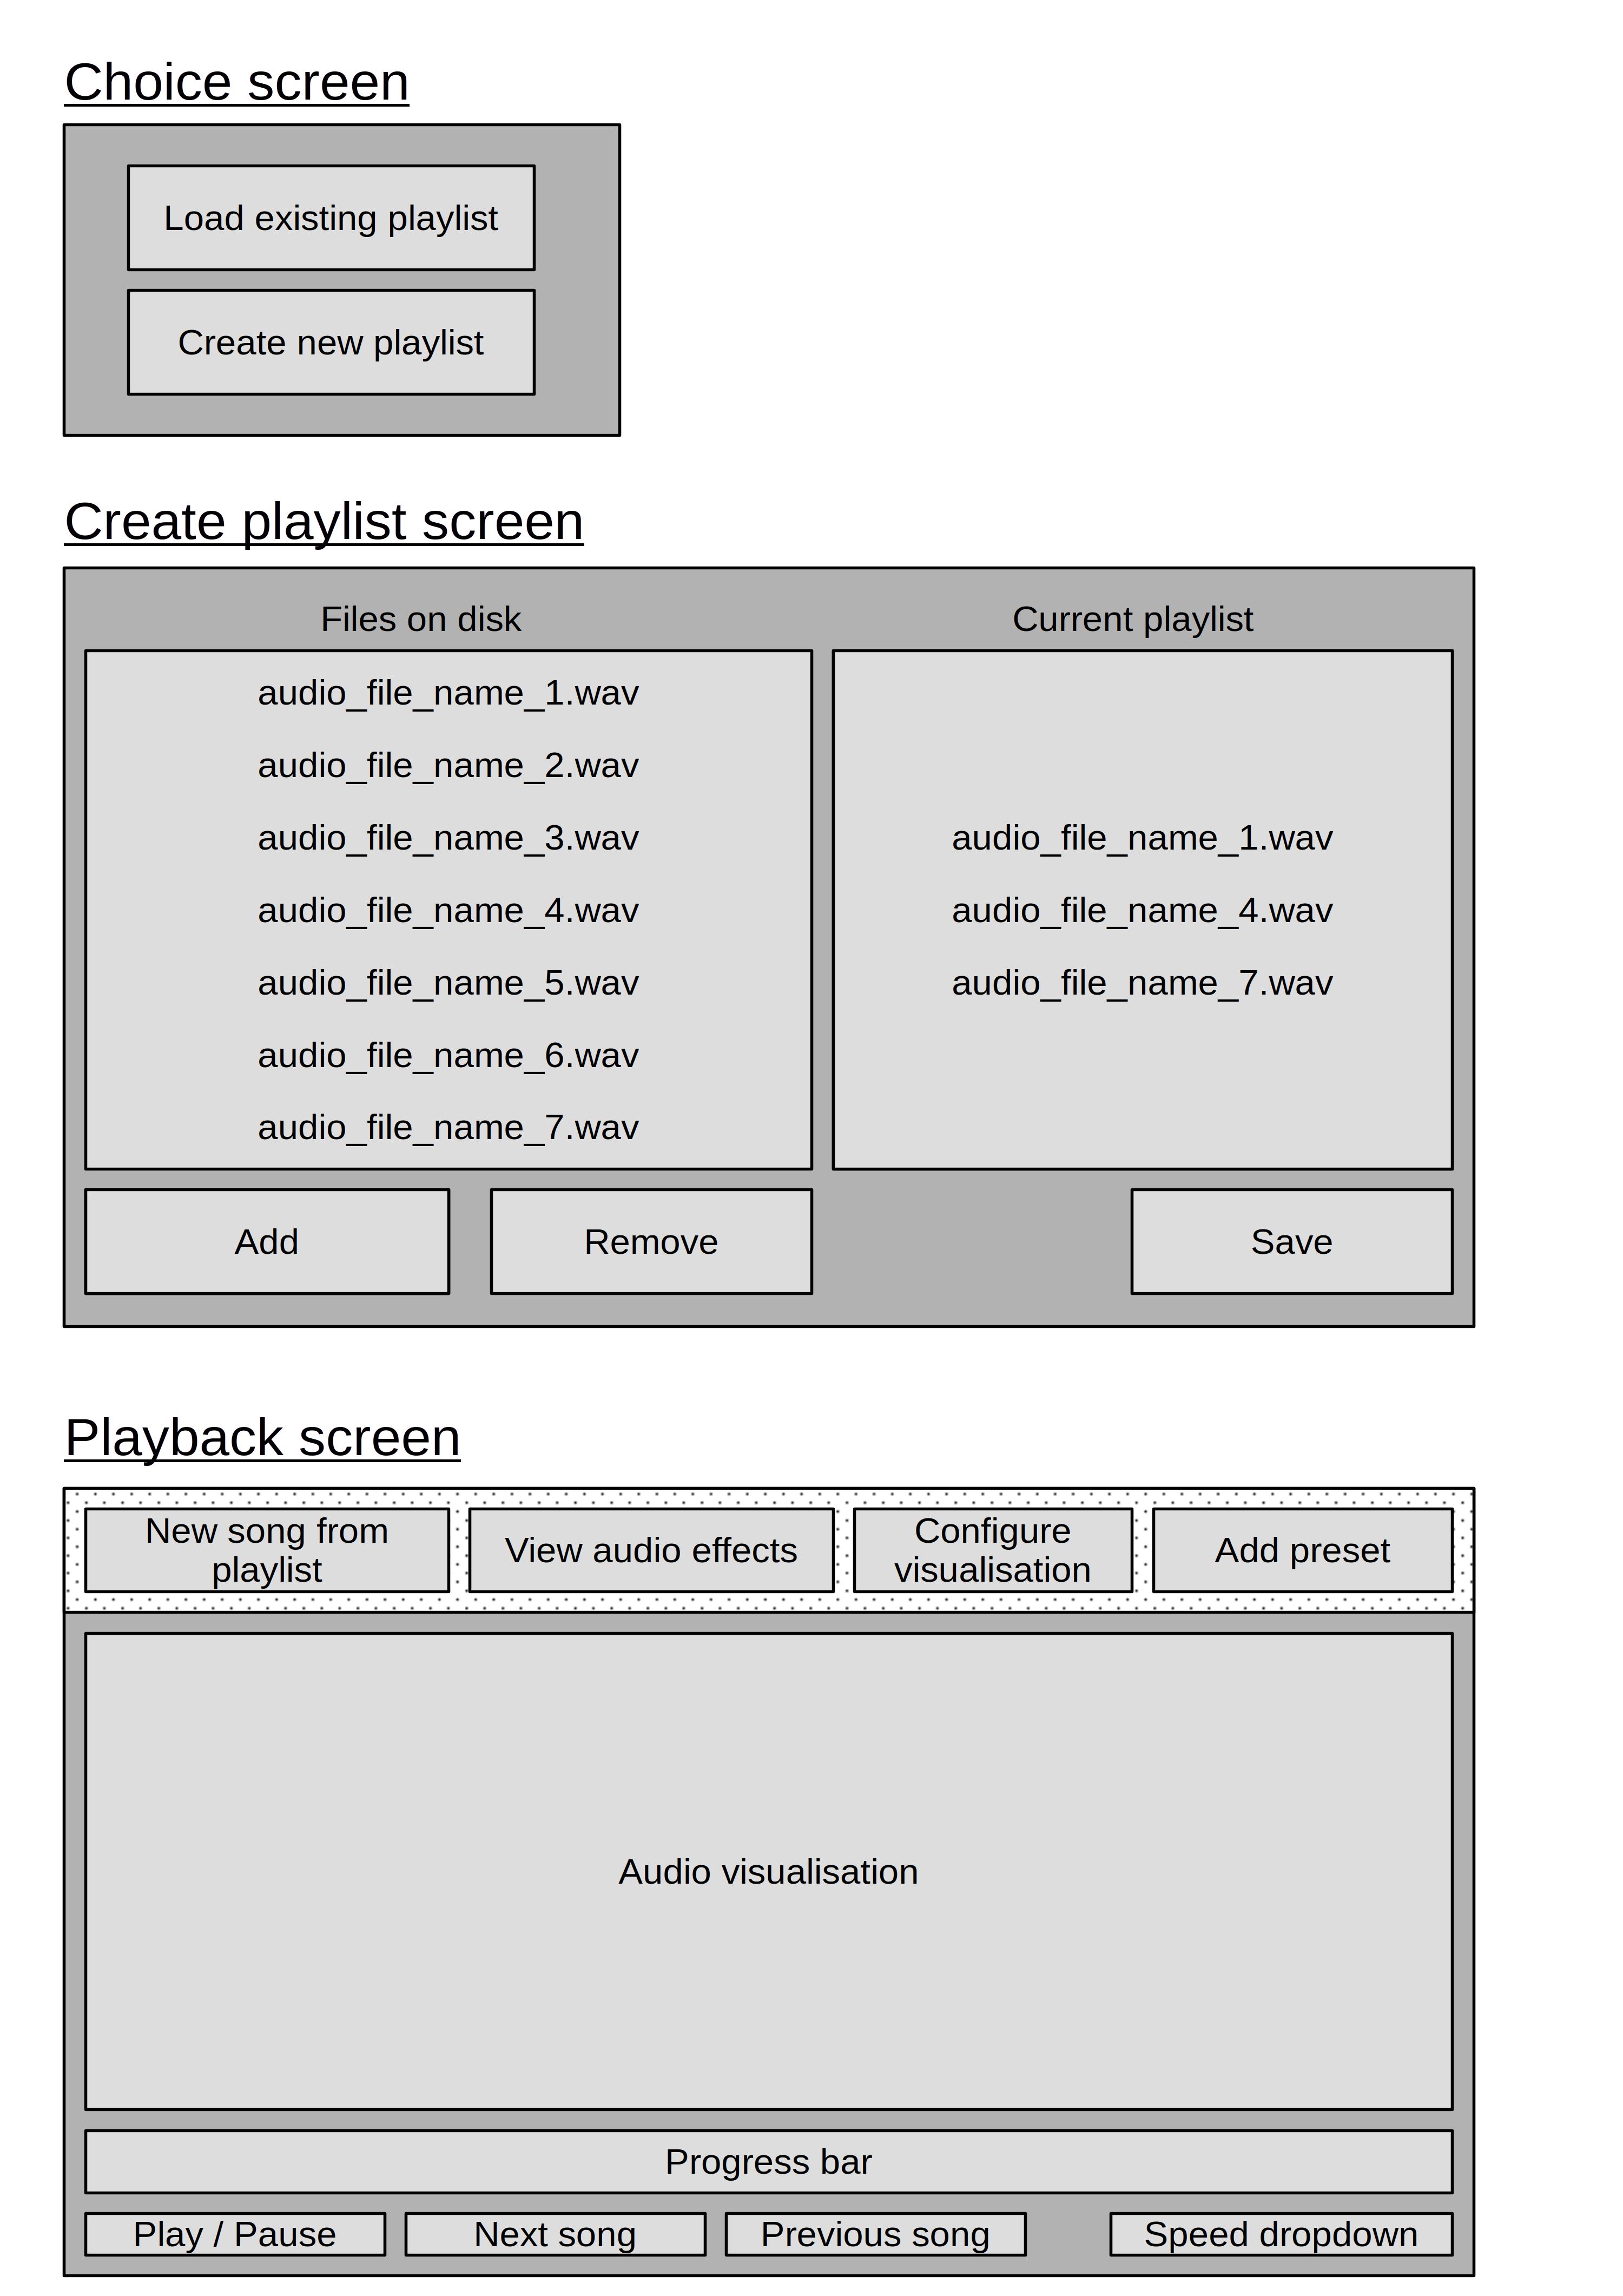
\includegraphics[width=14cm]{gui wireframes one}
	\caption{GUI wireframes for main windows }
\end{figure}

\begin{figure}[H]
	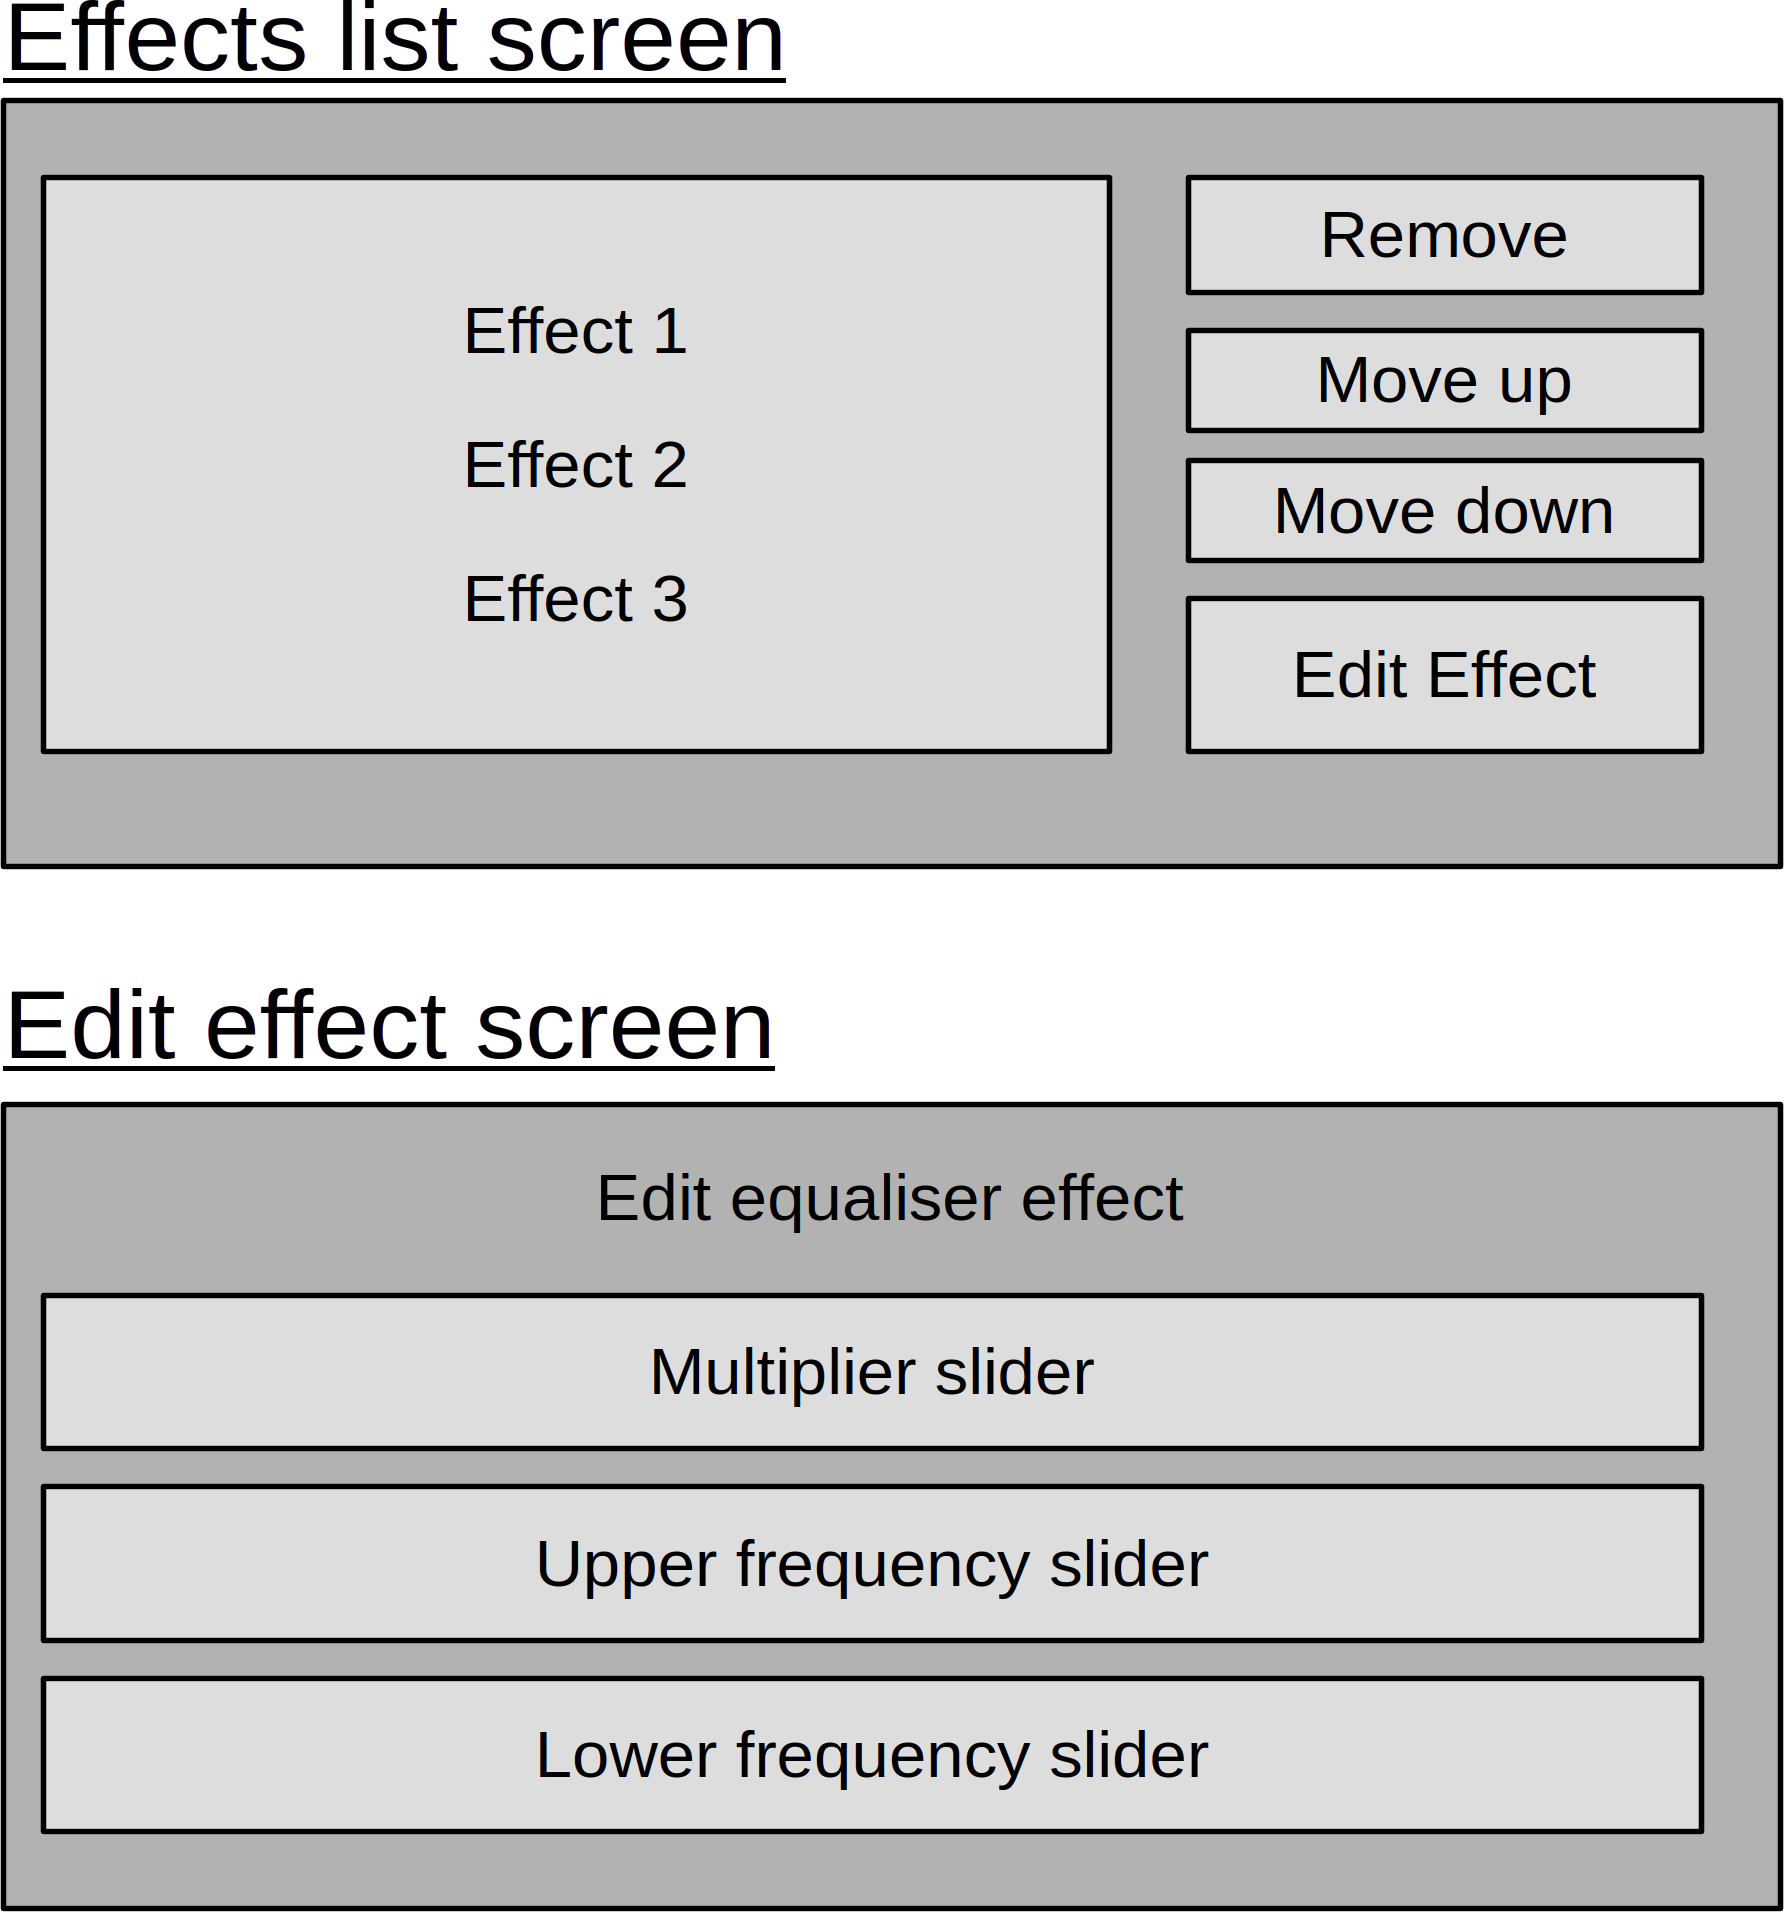
\includegraphics[width=14cm]{gui wireframes two}
	\caption{GUI wireframes for ancillary windows }
\end{figure}

\subsubsection{Relation to the Code}
As I am using "wxWidgets" (see above), all GUIs must be programmed directly in code. I have decided, therefore, to create the following classes to abstract away the details of the GUI:
\begin{itemize}
	\item StartupWindow - implements the initial "choice screen"
	\item PlaylistWindow - implements the "create playlist screen"
	\item FileBrowser - responsible for fetching and drawing the  list of audio files on the system (used by PlaylistWindow). This is abstracted away as "wxWidgets" does not provide a native "widget" for this, so I must create my own.
	\item PlayWindow - implements the "playback screen"
	\item EffectsWindow - implements the "effects list" screen
	\item PropertiesWindow - implements the "edit effect" screen
	\item SongSelectionWindow - draws the popup for when the user chooses to select a new song from the current playlist (abstracted as is non-trivial to implement)
\end{itemize}

\pagebreak
\subsection{Test Design}
\paragraph{}
In order to meet the objectives described in the analysis section, I have decided to design a variety of measurable tests which will indicate if these objectives have been met. For convenience, the objectives are repeated below:

\paragraph{}
{
	\centering
	\fbox{\begin{minipage}{15cm}
			
			\begin{enumerate}
				\item  The user must be able to load a collection of audio files known as a "playlist" and then play the audio files contained within in a logical order
				\item  The user must be able to visualise the current audio being played in the frequency domain (i.e. visualise the frequencies)
				\item The user must be able to modify the audio's frequency domain (i.e. selectively modify frequencies such as by performing a bass boost)
				\item The user must be able to apply additional "audio effects" to further enhance the music: echo, volume adjustment and noise
				\item The user must be able to configure these "audio effects" individually and also apply pre-made "presets" to quickly reach a desired effect
				\item  The system must run in real-time on an average school computer
			\end{enumerate}
			
	\end{minipage}}
}

\pagebreak
\subsubsection{Testing Objective 1}
\paragraph{Description} "The user must be able to load a collection of audio files known as a "playlist" and then play the audio files contained within in a logical order"

\paragraph{Test 1.1}
The user must have the option to create a new playlist from a list of audio files on the system.  To test this, I will therefore place a variety of audio files on disk and verify they are detected by the program.

\paragraph{Test 1.2}
I will then test if playlists created in the program can be successfully saved to disk, then loaded back into the program in a sanitised manner. In other words, playlists consisting solely of files which actually exist on disk should be loaded without error, but playlists with invalid audio files should fail to load and notify the user of the error.

\paragraph{Test 1.3}
After loading a playlist, the audio files contained within must appear "in a logical order", so I will verify that entries in the playlist are organised alphabetically, as is custom in audio programs.

\pagebreak
\subsubsection{Testing Objective 2}
\paragraph{Description} "The user must be able to visualise the current audio being played in the frequency domain (i.e. visualise the frequencies)"

\paragraph{}
As it is difficult for humans to visualise the frequency domain of audio themselves, I will generate audio files consisting of a sine wave of a constant, known frequency. Thus, when the frequency domain is visualised, there should be a single visual peak corresponding to the chosen frequency. By testing the visualisation in this manner across a range of frequencies, it should therefore be possible to deduce if the visualisation is correct.

\paragraph{}
Obviously the vast majority of audio being played will consist of multiple frequencies. I will therefore combine multiple sine waves in a single audio file (e.g. 500 Hz and 1000 Hz, both playing at the same time). Thus there should be multiple identifiable peaks, each one corresponding to a sine wave frequency chosen.

\paragraph{}
It should be stressed that human hearing only extends from 20 Hz to 20,000 Hz, and as such any audio visualisation must exclude frequencies outside these ranges.

\begin{figure}[H]
	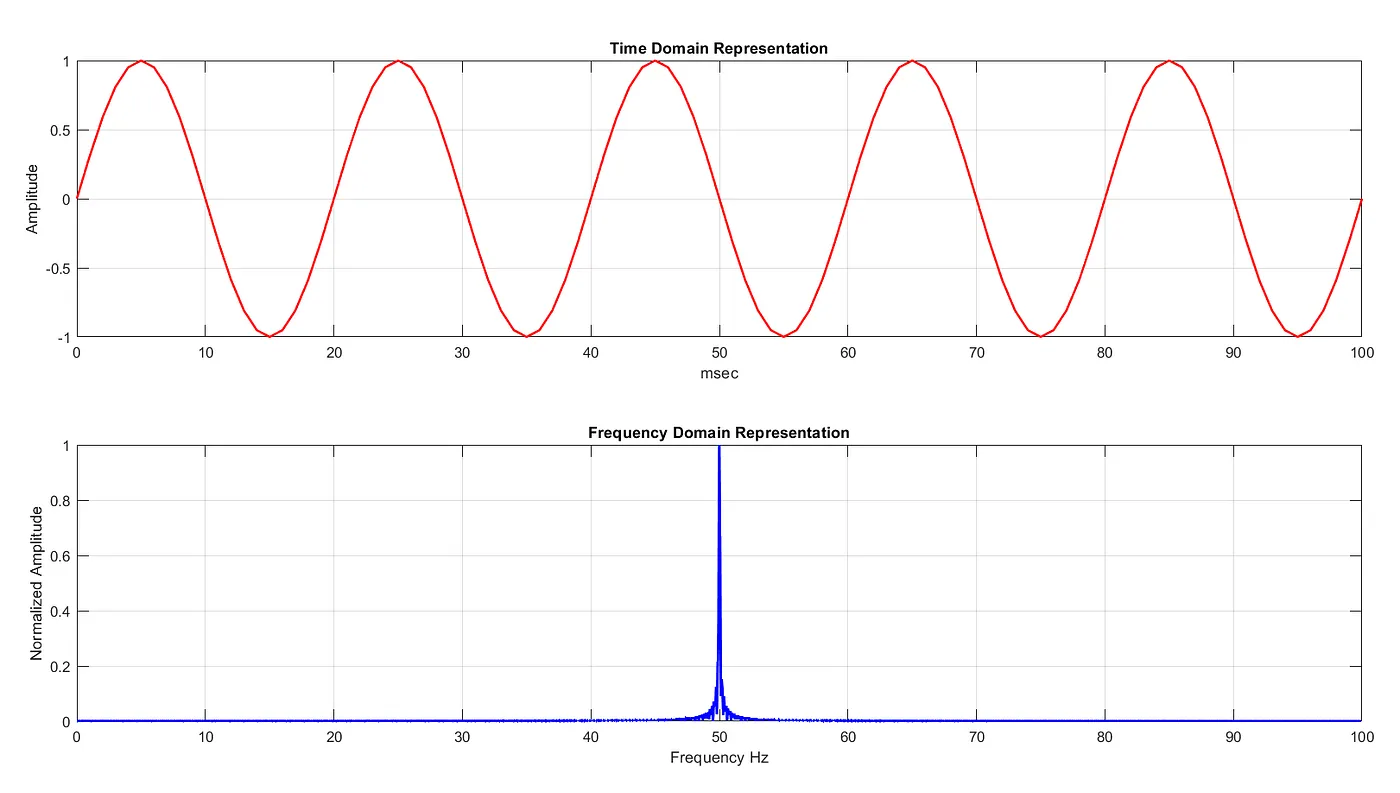
\includegraphics[width=14cm]{fft test example}
	\caption{An example piece of audio, with the time domain shown above and the frequency domain below. If my tests succeed, they should look similar to the first picture (multiple sine waves will of course have multiple peaks of this nature). }
	% Credit - Aniket Kamat: https://aniket-kamat.medium.com/demystifying-the-fourier-transform-a995bdb6d73a
\end{figure}

\paragraph{Test 2.1} A correct visualisation of a sine wave is apparent at 500 Hz, with a single peak corresponding to that frequency.
\paragraph{Test 2.2} A correct visualisation of a sine wave is apparent at 1,000 Hz, with a single peak corresponding to that frequency.
\paragraph{Test 2.3} Sine waves outside the human audible range, at 10 Hz and 100,000 Hz respectively, produce no visible output, as they are inaudible.
\paragraph{Test 2.4} A correct visualisation of two sine waves (one at 1,000 Hz and one at 10,000 Hz) is apparent, with two separate peaks corresponding to those frequencies.
\paragraph{Test 2.5} A correct visualisation of three sine waves (1,000 Hz, 5,000 Hz and 20,000 Hz ) is apparent, with three separate peaks corresponding to those frequencies.

\pagebreak
\subsubsection{Testing Objective 3}
\paragraph{Description} "The user must be able to modify the audio's frequency domain (i.e. selectively modify frequencies such as by performing a bass boost)"

\paragraph{Test 3.1}
The most common use case for this feature will be when adjusting the bass and treble of music. I will therefore play multiple songs in the program with the equaliser effect applied, and verify by ear that the program is able to selectively reduce the range of frequencies chosen.

\paragraph{Test 3.2}
As a sanity test, I will also ensure that changes made to the audio's frequency domain are clearly visible in the audio visualisation.\footnote{
	For example, if one chooses to reduce the bass, then the parts
	of the visualisation corresponding to the lower frequencies must
	visually appear smaller in relation to the other frequencies.
}

\pagebreak
\subsubsection{Testing Objective 4}
\paragraph{Description} "The user must be able to apply additional "audio effects" to further enhance the music: echo, volume adjustment and noise"

\paragraph{}
Due to the subjective nature of audio effects, I will ask multiple people from the program's target audience to provide in-depth feedback on all the audio effects.
At least one of these people will be someone experienced in audio processing, so that they are able to assess if the effects provided sound physically accurate
(particularly the echo).

\paragraph{Test 4.1} A select group from the target audience certify that the echo effect sounds physically plausible
\paragraph{Test 4.2} A select group from the target audience certify  that the noise effect sounds physically plausible
\paragraph{Test 4.3} A select group from the target audience certify that the volume effect adjusts the volume correctly

\pagebreak
\subsubsection{Testing Objective 5}
\paragraph{Description} "The user must be able to configure these "audio effects" individually and also apply pre-made "presets" to quickly reach a desired effect"

\paragraph{Test 5.1} All presets present in the application can be loaded successfully and results in the desired effects being applied correctly
\paragraph{Test 5.2} All effects can have their various parameters modified, which results in a correct change in the audio playback

\pagebreak
\subsubsection{Testing Objective 6}
\paragraph{Description}  "The system must run in real-time on an average school computer"

\paragraph{}
I will test the performance of the program by running it on a computer in my school, which represents more-or-less average hardware.
I will also test it on my school laptop too, which has more modest hardware, to ensure that in all contexts in which a student might run the program, there will be no performance issues.
In order to appear to run in real-time, the following must be observed:
\begin{enumerate}
	\item The audio  playback must not slow down \footnote{If audio processing takes too long, then the audio callback will be called less frequently than the hardware demands, resulting
		in a very noticeable slowdown. This must not happen.}.
	\item The visualisation graphics must update in less than 16.6 ms, such that it is displayed at 60 FPS, which is the most common refresh rate on school hardware. This will be measured by
	the code itself as it's running.
\end{enumerate}

\paragraph{Test 6.1} The program must run, without any effects applied, in real-time on the specified hardware
\paragraph{Test 6.2} The program must run in real-time, for every preset applied separately, in real-time on the specified hardware.  
\paragraph{Test 6.3} The program must run in real-time, with every effect applied at once, in real-time on the specified hardware.  

\pagebreak
\subsection{Final overview of project hierarchy}
\begin{figure}[H]
	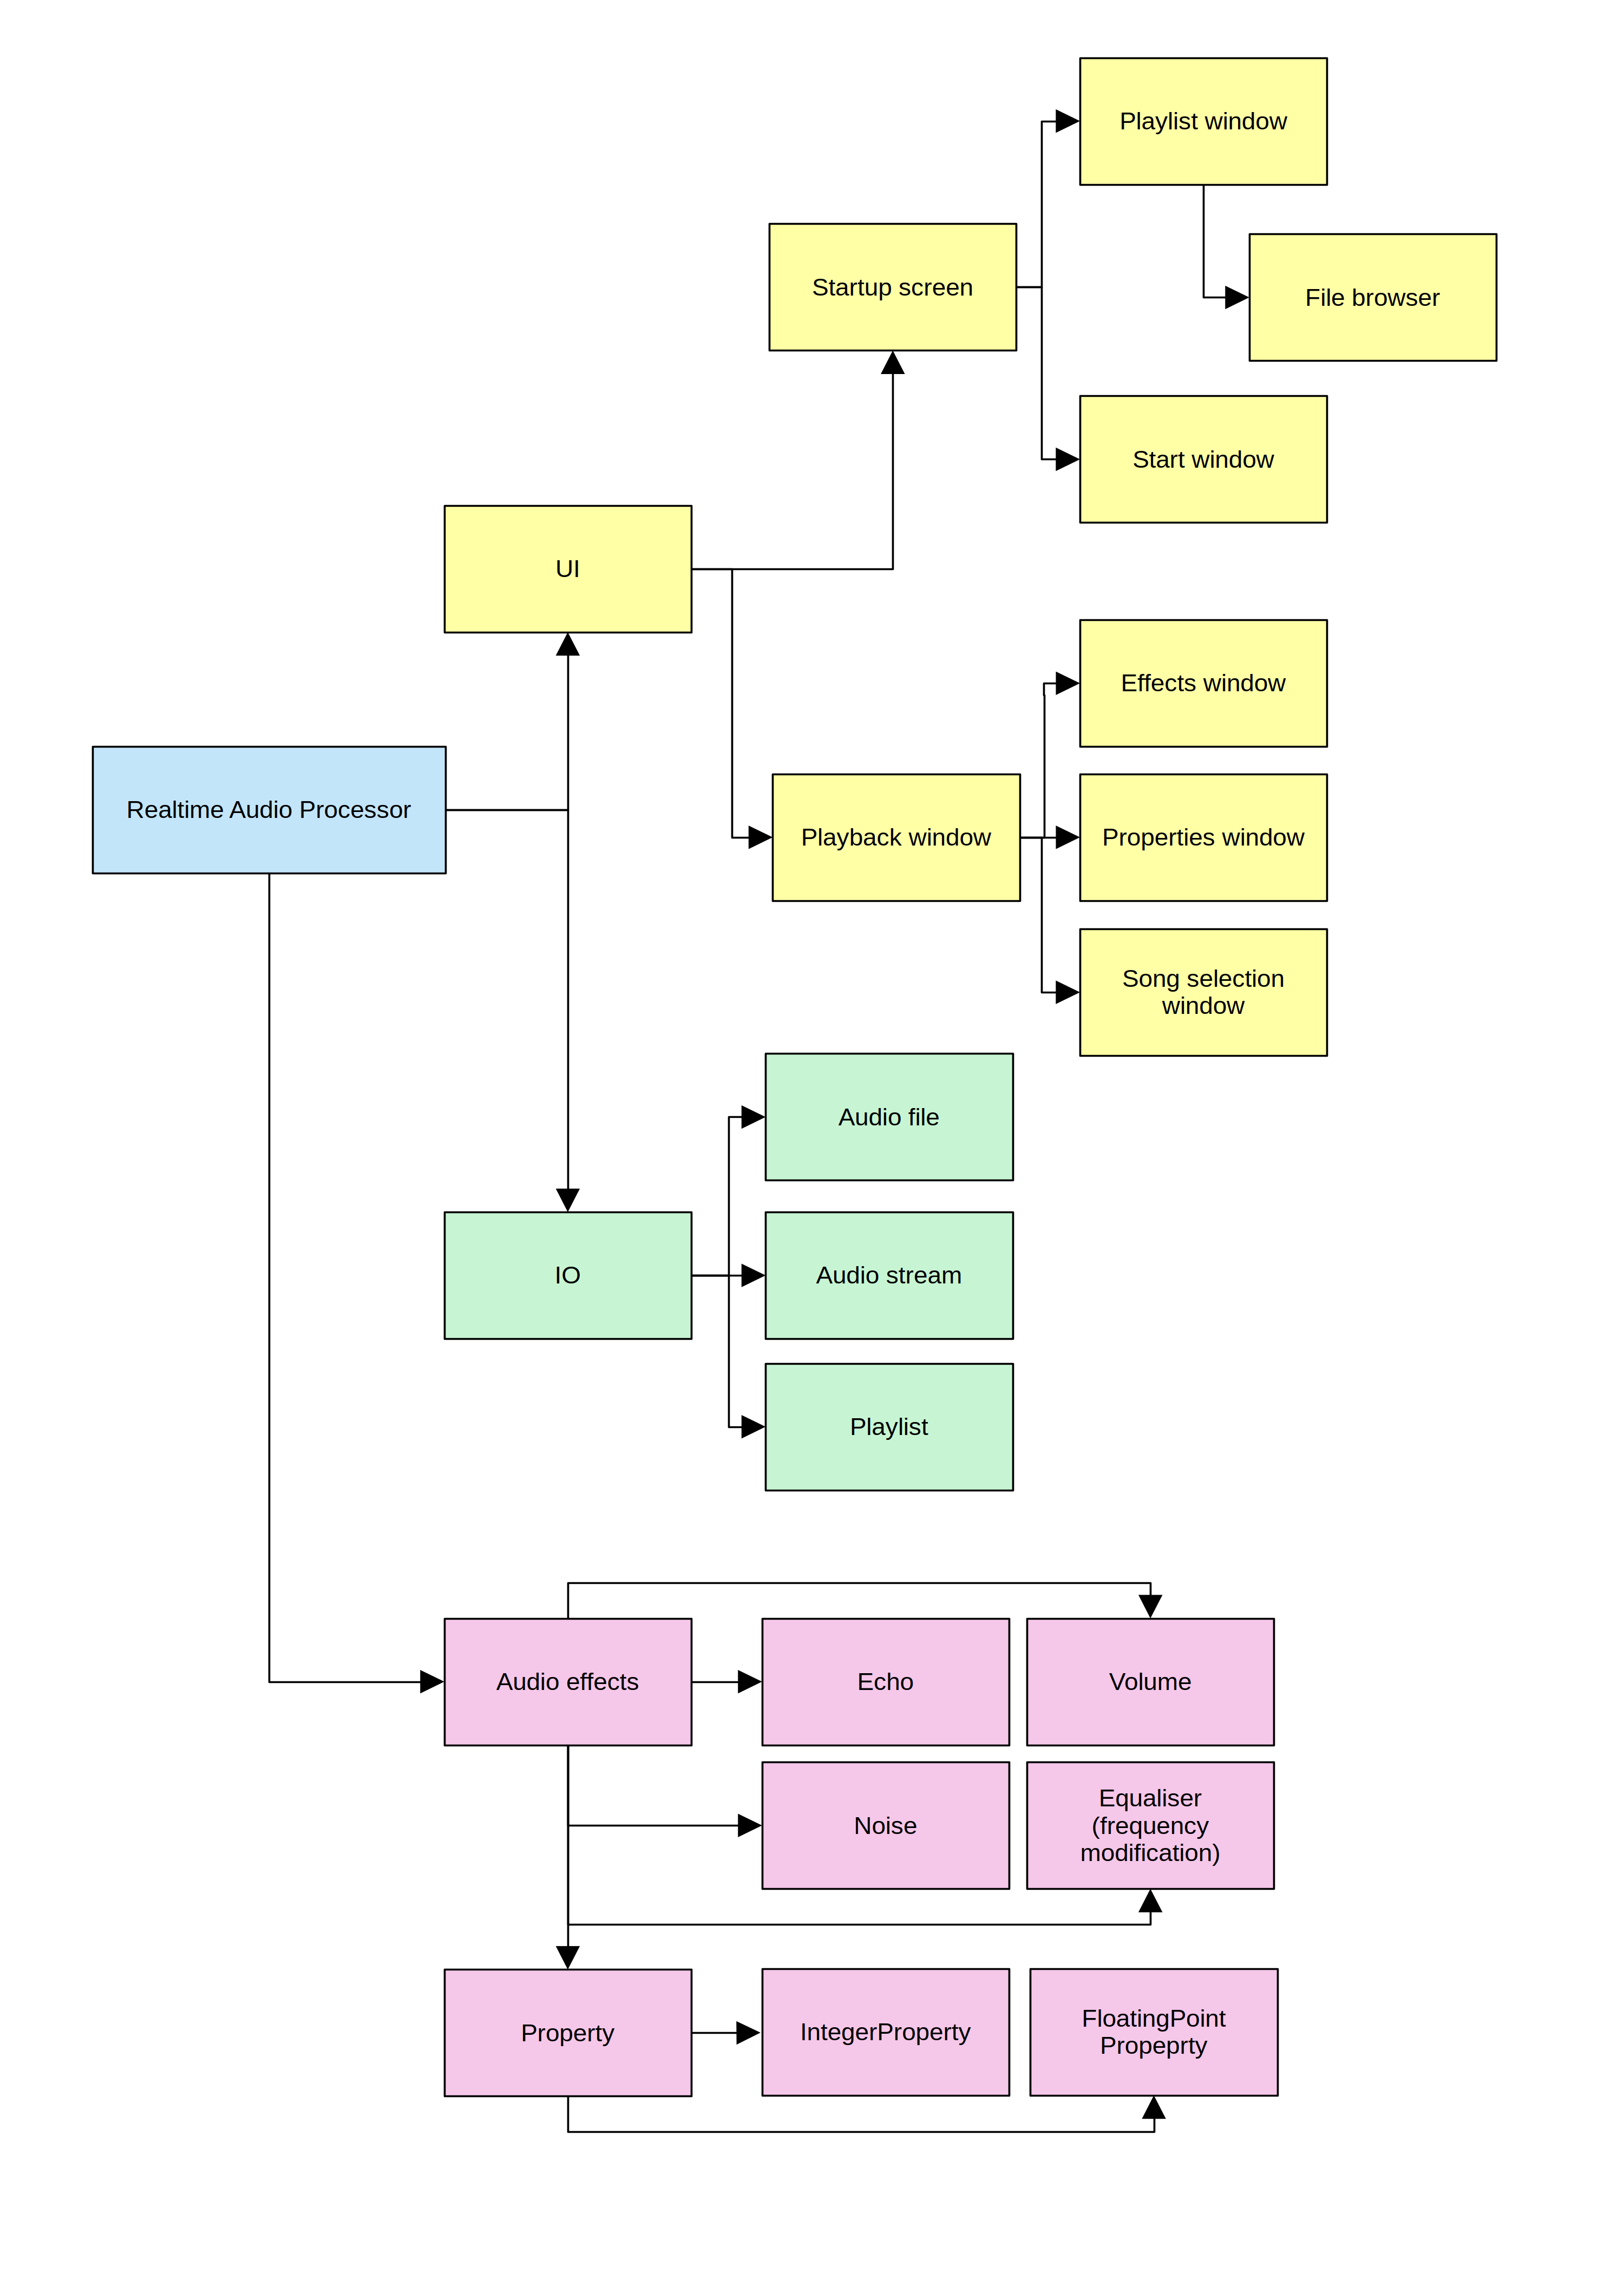
\includegraphics[width=14cm]{hierarchy chart}
	\caption{Hierarchy chart }
\end{figure}
